% для компиляции в lualatex!!
%\documentclass[12pt, a4paper]{article}
\documentclass[12pt, a4paper]{disser}
\usepackage[english,russian]{babel}
\usepackage[warn]{mathtext}
%\usepackage[T2A]{fontenc}
%\usepackage[utf8]{inputenc}

\usepackage{xecyr} % Продукт Вашего покорного слуги ;)

%\setmainfont{DejaVu Serif}
\setmainfont{Liberation Serif}

\usepackage{color}
\usepackage{amssymb,amsmath}
\usepackage{graphicx}
\usepackage{multicol}

\textheight=24cm           % высота текста
\textwidth=16cm            % ширина текста
\oddsidemargin=0pt         % отступ от левого края
\topmargin=-1.5cm          % отступ от верхнего края
\parindent=24pt            % абзацный отступ
\parskip=0pt               % интервал между абзацами
\tolerance=2000            % терпимость к "жидким" строкам
\flushbottom               % выравнивание высоты страниц
%\def\baselinestretch{1.5} % печать с большим интервалом

%\title{}
%\author{\copyright~~С.А.~Назарова \thanks{e-mail:~sophia.nazarova@gmail.com}}
%\date{}


\begin{document}
	
	\begin{figure}[h]

	\begin{minipage}[b]{.46\linewidth}
%Фигурка в первом ряду слева размер отведенный под весь этот объект \textendash 0.46 от ширины строки
%Параметр [b] означает, что выравнивание этих министраниц будет по нижнему краю
	\begin{center}
	{\small N~{\it Macoma balthica}}
		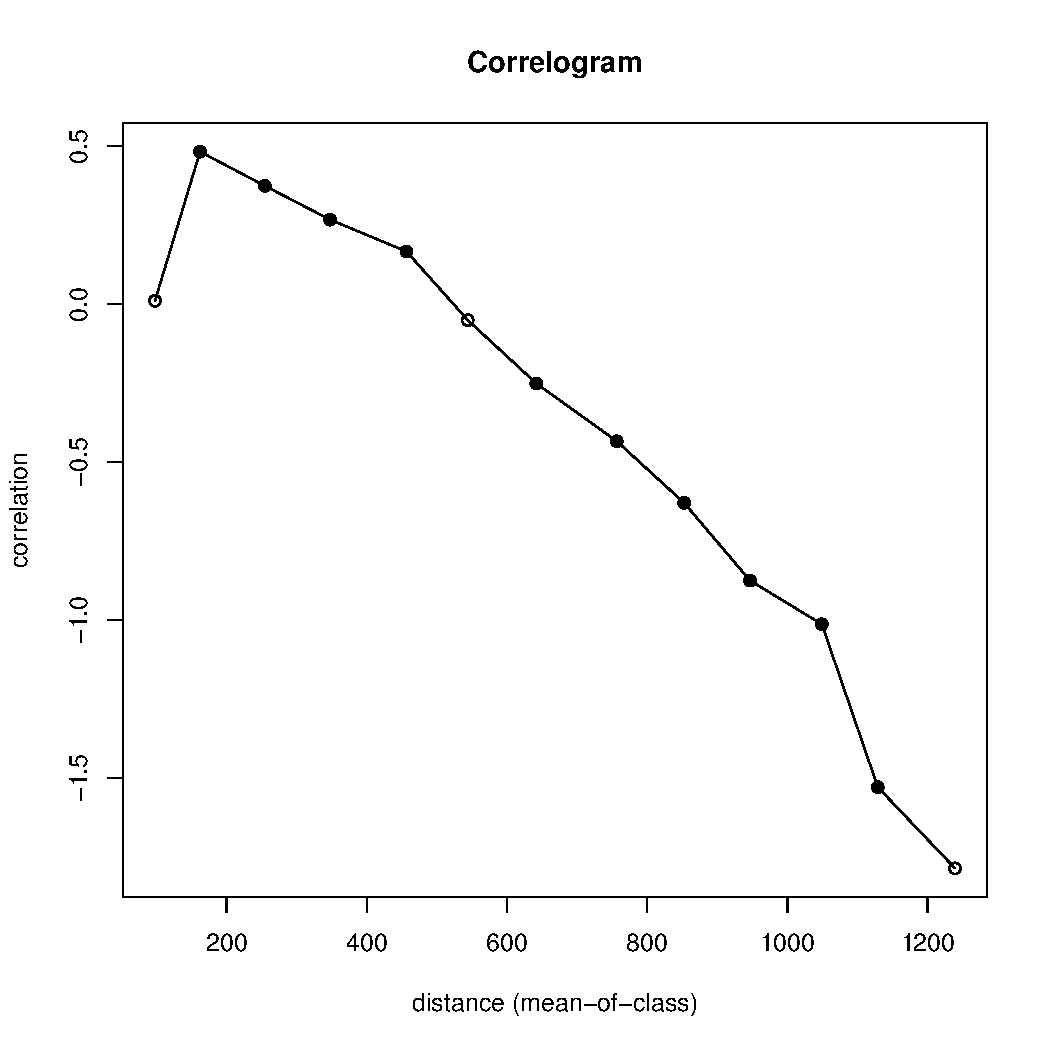
\includegraphics[width=65mm]{../Barenc_Sea/distribution_Moran/Pala_moran_N_Macoma_balthica_.pdf}
	\end{center}
	\end{minipage}
%
	\hfil %Это пружинка отодвигающая рисунки друг от друга
%
	\begin{minipage}[b]{.46\linewidth}
%Следующий рисунок - первый ряд справа %DUNGEON S_4 \ AB
	\begin{center}
	{\small B~{\it Macoma balthica}}
		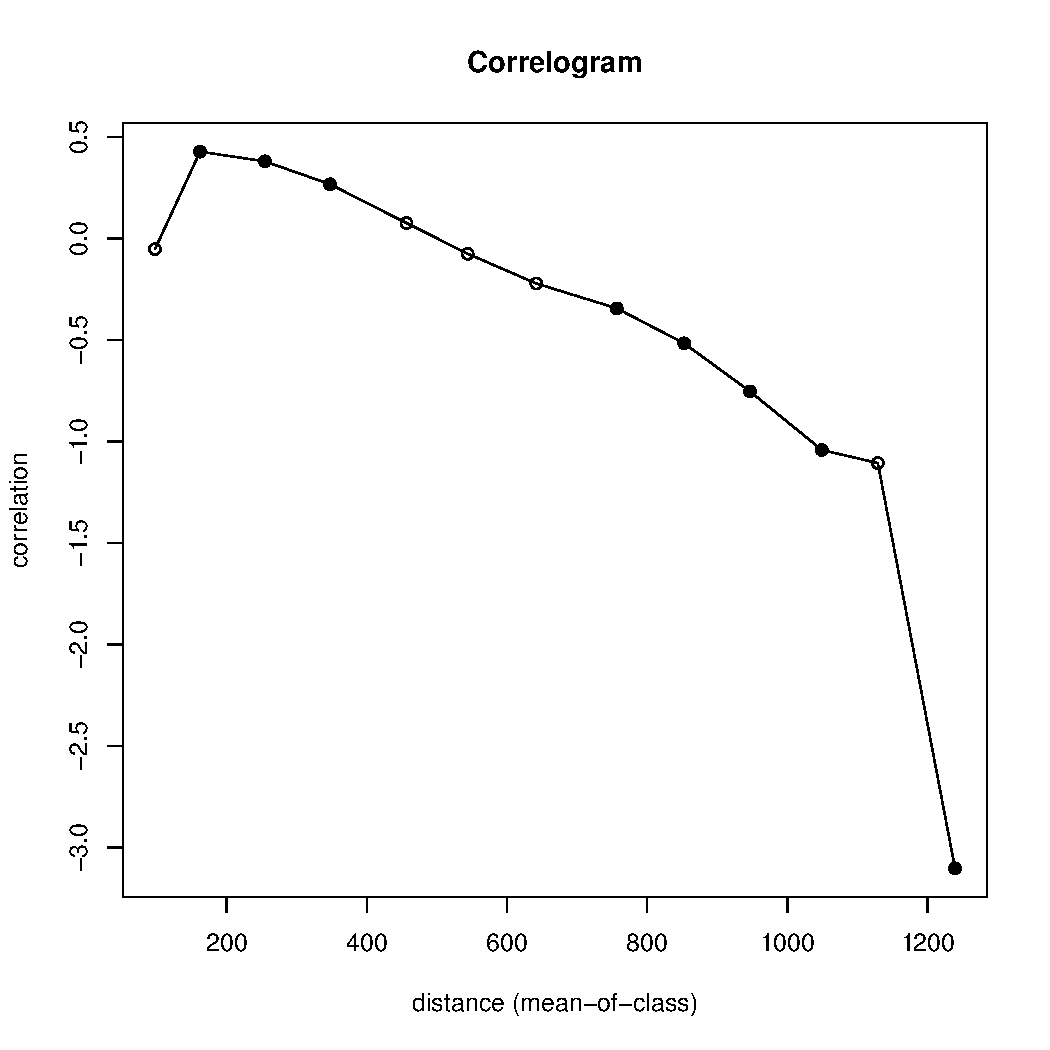
\includegraphics[width=65mm]{../Barenc_Sea/distribution_Moran/Pala_moran_B_Macoma_balthica_.pdf}
	\end{center}
	\end{minipage}

	
	\begin{minipage}[b]{.46\linewidth}
	%Фигурка в первом ряду слева размер отведенный под весь этот объект \textendash 0.46 от ширины строки
	%Параметр [b] означает, что выравнивание этих министраниц будет по нижнему краю
	\begin{center}
	{\small N~{\it Cerastoderma edule}}
		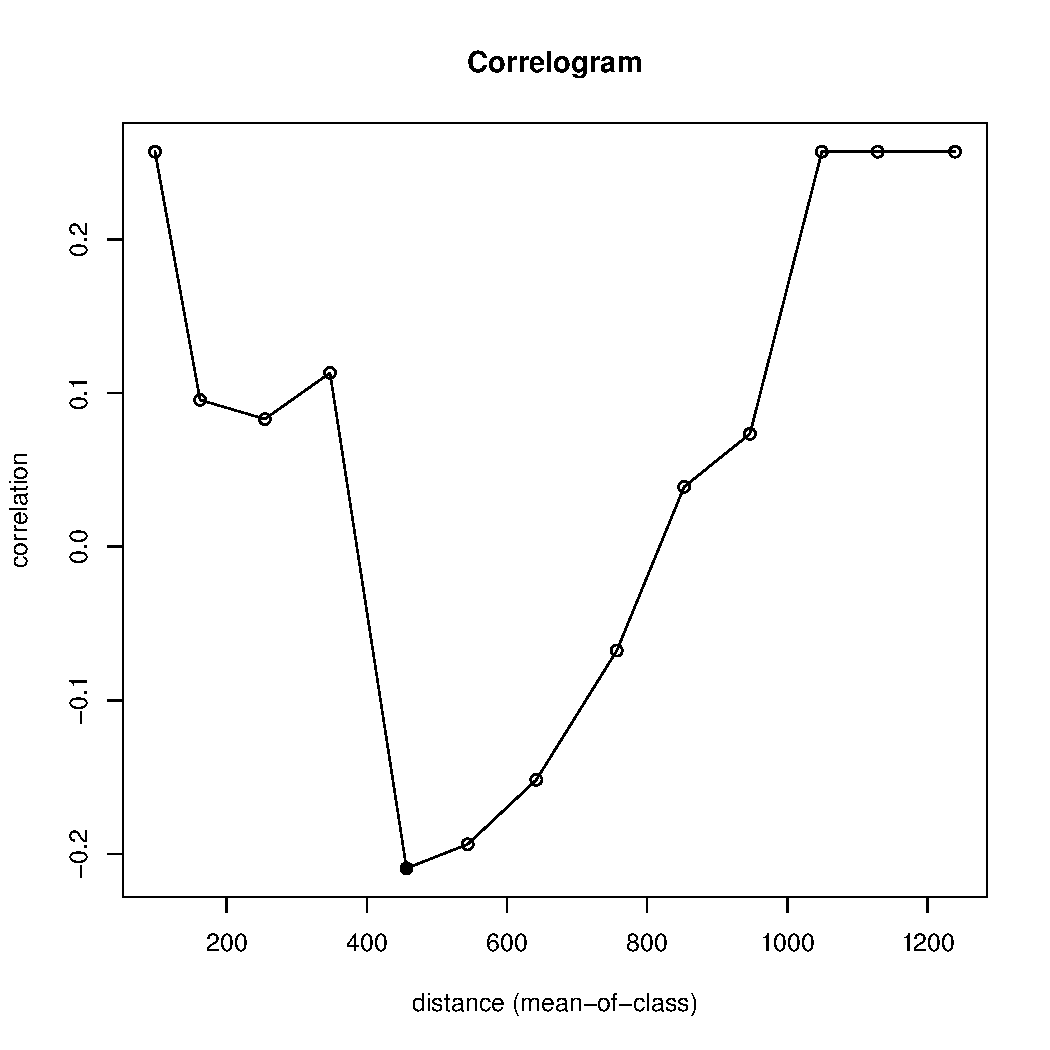
\includegraphics[width=65mm]{../Barenc_Sea/distribution_Moran/Pala_moran_N_Cerastoderma_edule_.pdf}
	\end{center}
	\end{minipage}
	%
	\hfil %Это пружинка отодвигающая рисунки друг от друга
	%
	\begin{minipage}[b]{.46\linewidth}
%Следующий рисунок - первый ряд справа %DUNGEON S_4 \ AB
	\begin{center}
	{\small B~{\it Cerastoderma edule}}
		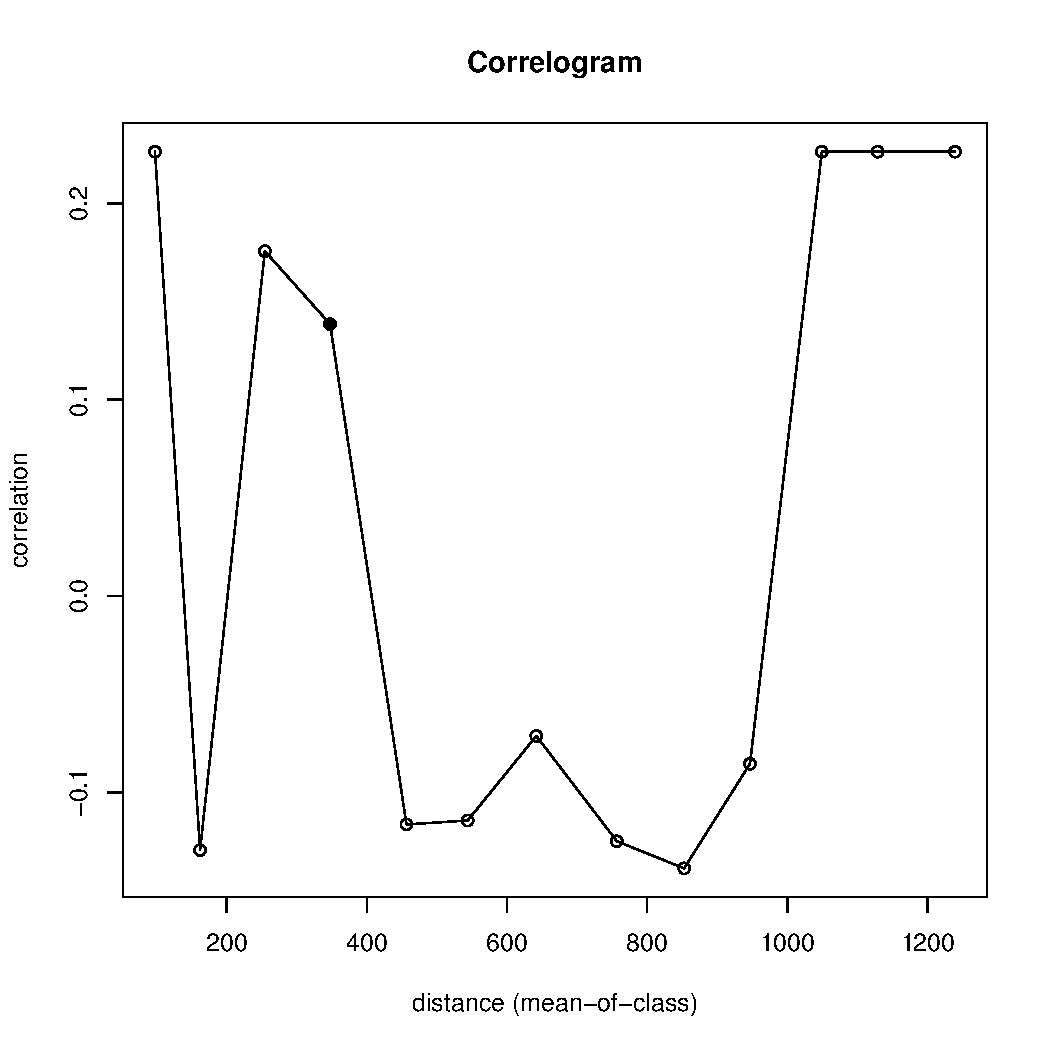
\includegraphics[width=65mm]{../Barenc_Sea/distribution_Moran/Pala_moran_B_Cerastoderma_edule_.pdf}
	\end{center}
	\end{minipage}

%\smallskip



%\smallskip

	\begin{minipage}[b]{.46\linewidth}
%Фигурка в первом ряду слева размер отведенный под весь этот объект \textendash 0.46 от ширины строки
%Параметр [b] означает, что выравнивание этих министраниц будет по нижнему краю
	\begin{center}
	{\small N~{\it Priapulus caudatus}}
		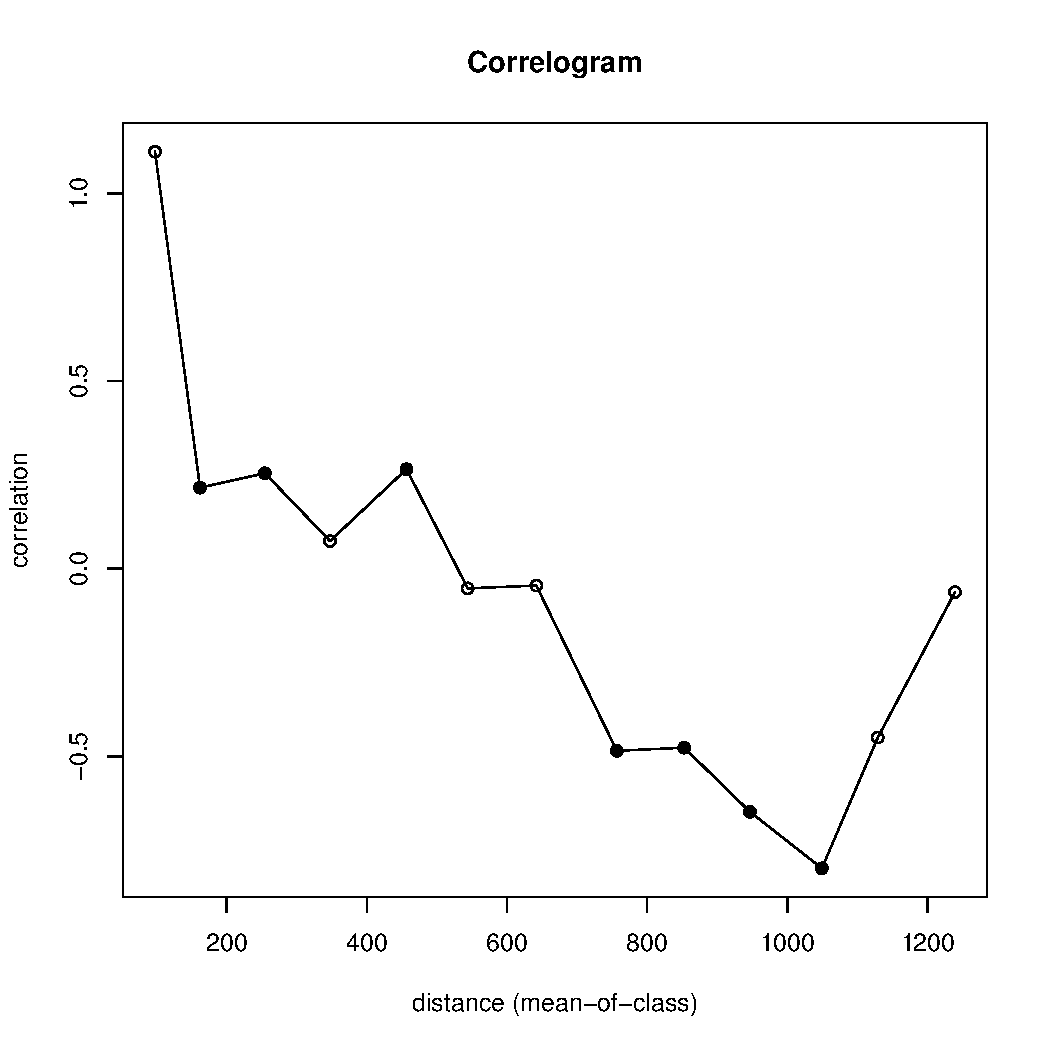
\includegraphics[width=65mm]{../Barenc_Sea/distribution_Moran/Pala_moran_N_Priapulus_caudatus_.pdf}
	\end{center}
	\end{minipage}
%
	\hfil %Это пружинка отодвигающая рисунки друг от друга
%
	\begin{minipage}[b]{.46\linewidth}
%Следующий рисунок - первый ряд справа %DUNGEON S_4 \ AB
	\begin{center}
	{\small B~{\it Priapulus caudatus}}
		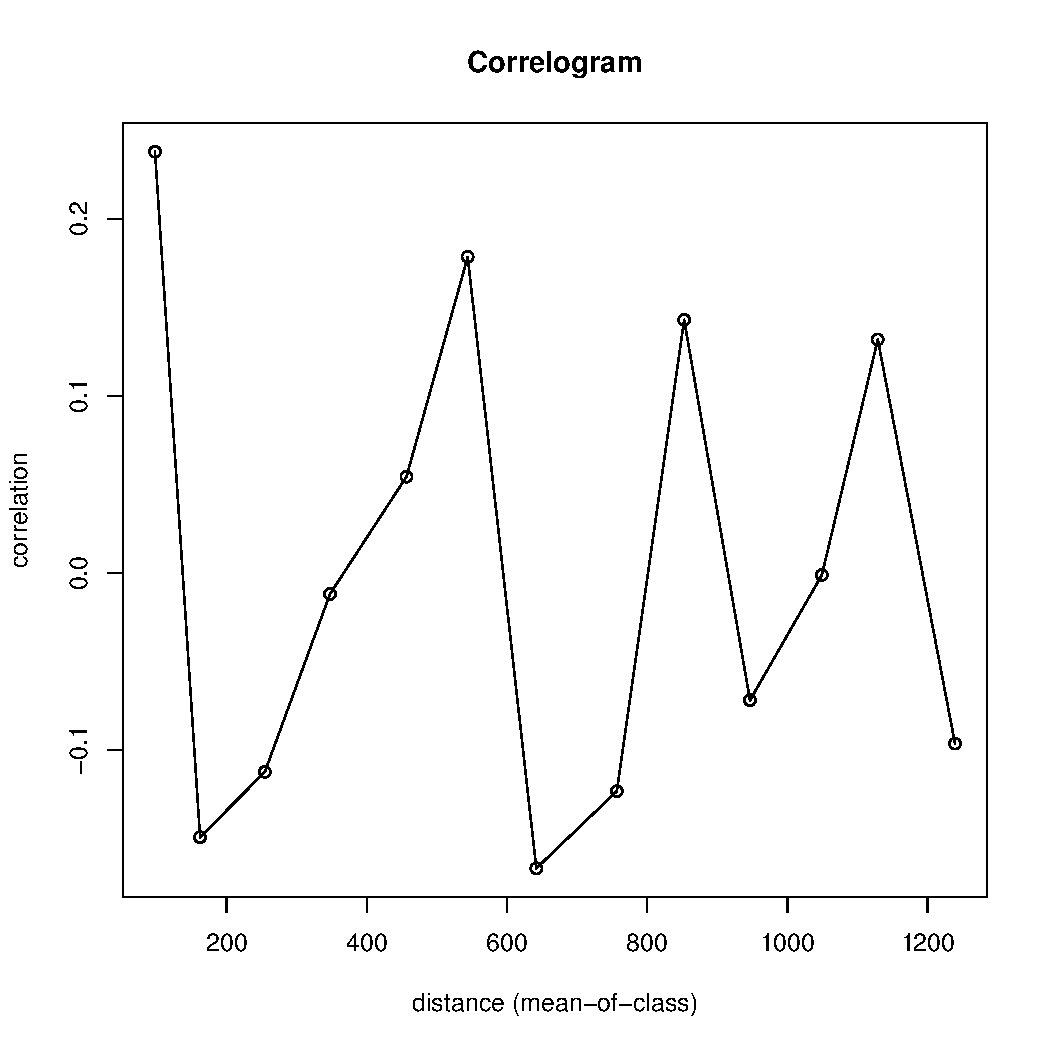
\includegraphics[width=65mm]{../Barenc_Sea/distribution_Moran/Pala_moran_B_Priapulus_caudatus_.pdf}
	\end{center}
	\end{minipage}

%\smallskip


	\caption{Микрораспределение макробентоса на литорали Пала-губы}
	\label{ris:moransI_Pala}
	\end{figure}



	\begin{figure}[h]

	\begin{minipage}[b]{.46\linewidth}
%Фигурка в первом ряду слева размер отведенный под весь этот объект \textendash 0.46 от ширины строки
%Параметр [b] означает, что выравнивание этих министраниц будет по нижнему краю
	\begin{center}
	{\small N~{\it Crangon crangon}}
		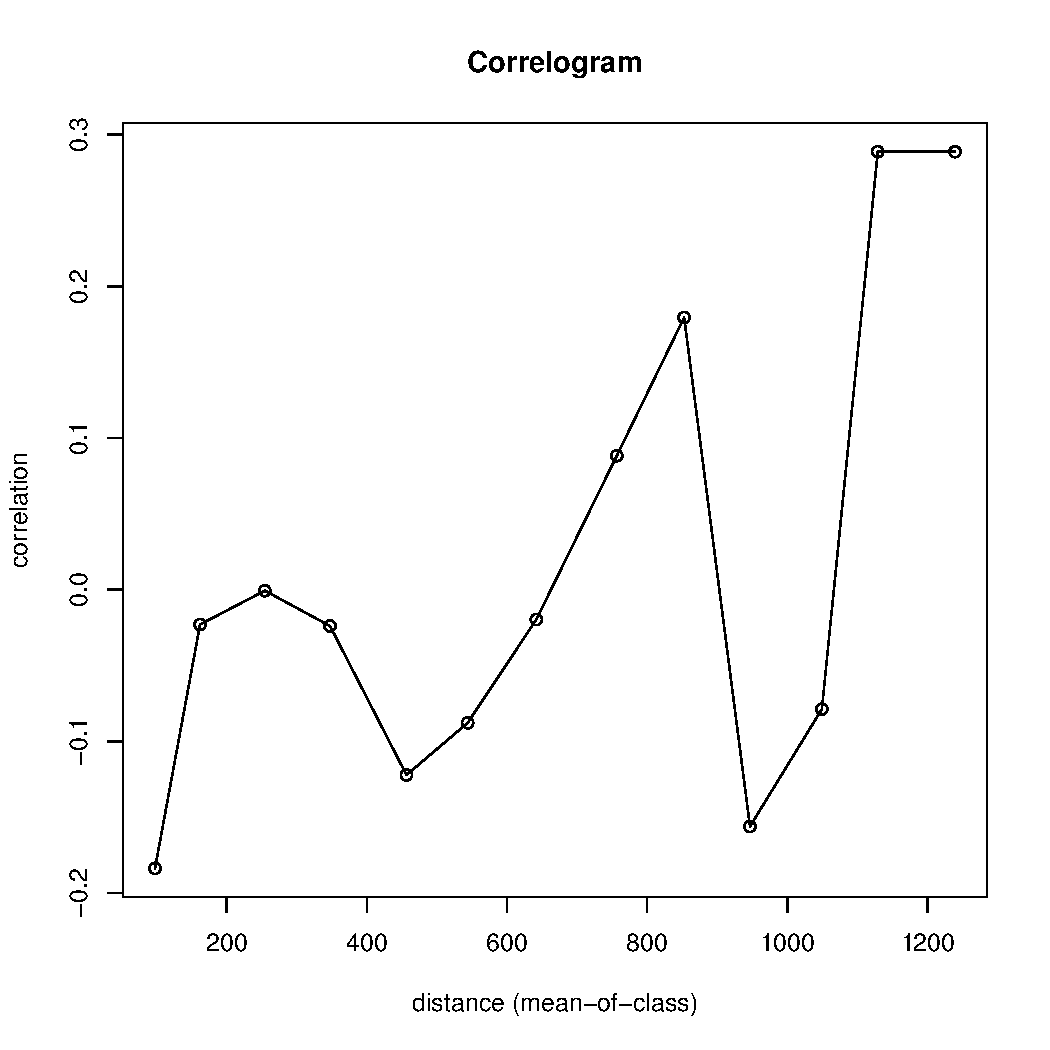
\includegraphics[width=65mm]{../Barenc_Sea/distribution_Moran/Pala_moran_N_Crangon_crangon_.pdf}
	\end{center}
	\end{minipage}
%
%	\hfil %Это пружинка отодвигающая рисунки друг от друга
%
%	\begin{minipage}[b]{.46\linewidth}
%Следующий рисунок - первый ряд справа %DUNGEON S_4 \ AB
%	\begin{center}
%		\includegraphics[width=65mm]{../Barenc_Sea/distribution_Moran/}
%	{\small B~{\it Crangon crangon}}
%	\end{center}
%	\end{minipage}

	
%	\begin{minipage}[b]{.46\linewidth}
	%Фигурка в первом ряду слева размер отведенный под весь этот объект \textendash 0.46 от ширины строки
	%Параметр [b] означает, что выравнивание этих министраниц будет по нижнему краю
%	\begin{center}
%	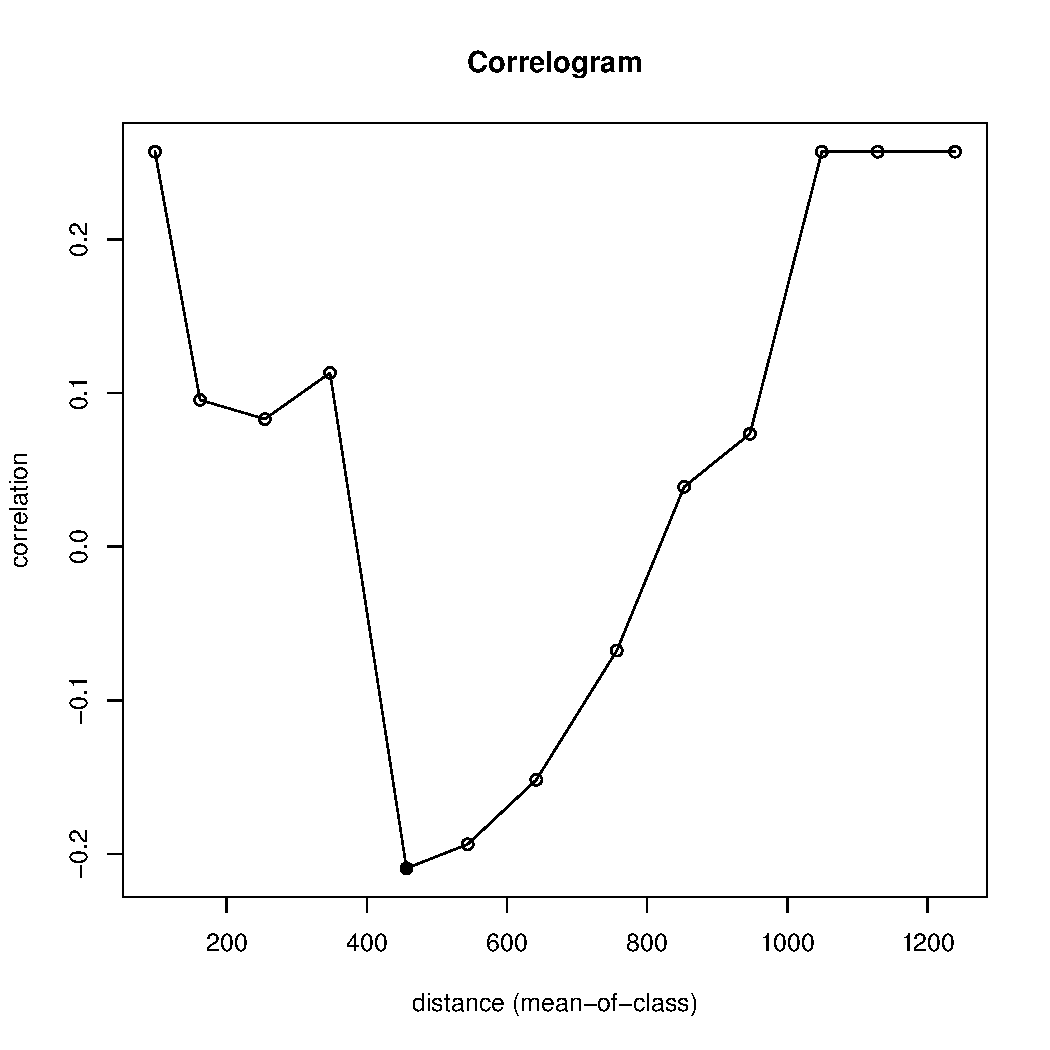
\includegraphics[width=65mm]{../Barenc_Sea/distribution_Moran/Pala_moran_N_Cerastoderma_edule_.pdf}

%	\end{center}
%	\end{minipage}
	%
%	\hfil %Это пружинка отодвигающая рисунки друг от друга
	%
%	\begin{minipage}[b]{.46\linewidth}
%Следующий рисунок - первый ряд справа %DUNGEON S_4 \ AB
%	\begin{center}
%		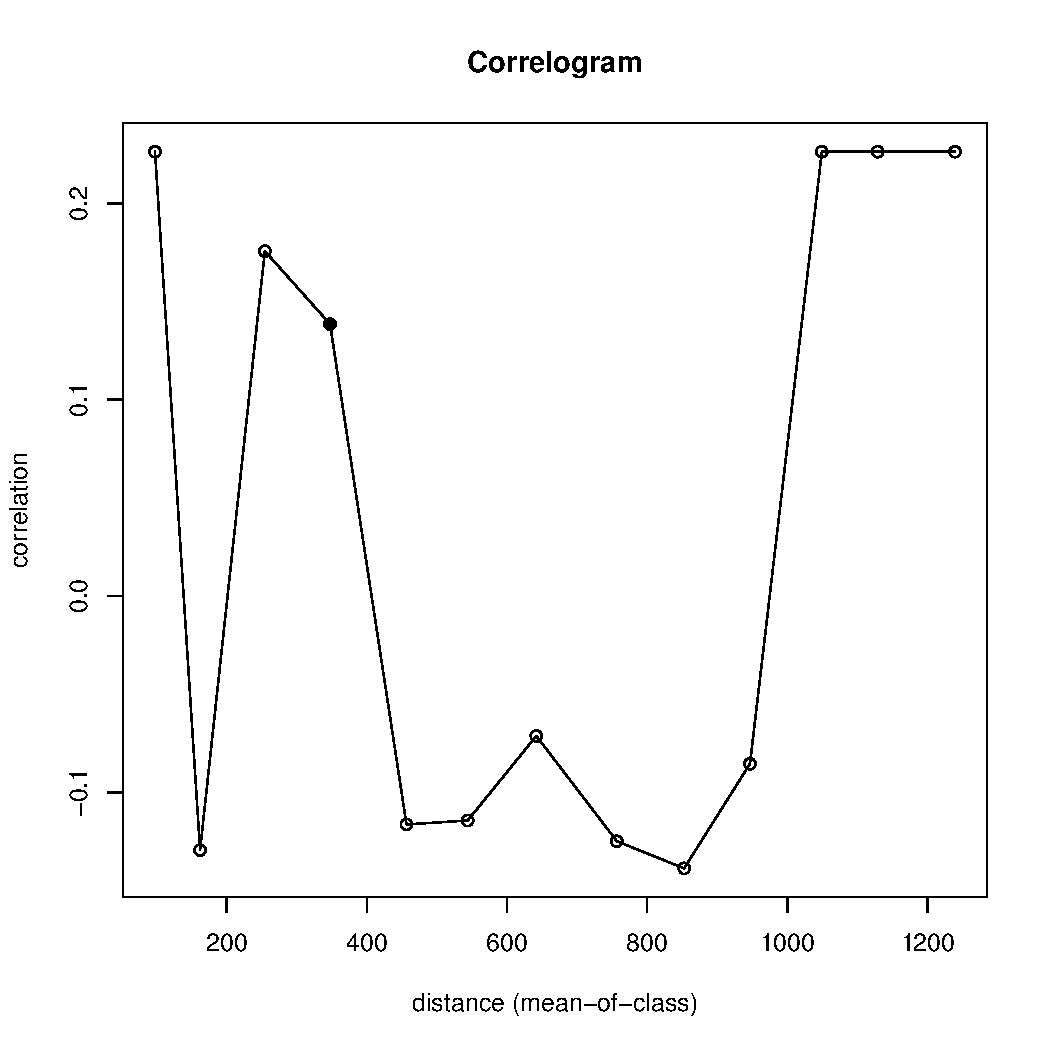
\includegraphics[width=65mm]{../Barenc_Sea/distribution_Moran/Pala_moran_B_Cerastoderma_edule_.pdf}
%	\end{center}
%	\end{minipage}

%\smallskip



%\smallskip

%	\begin{minipage}[b]{.46\linewidth}
%Фигурка в первом ряду слева размер отведенный под весь этот объект \textendash 0.46 от ширины строки
%Параметр [b] означает, что выравнивание этих министраниц будет по нижнему краю
%	\begin{center}
%		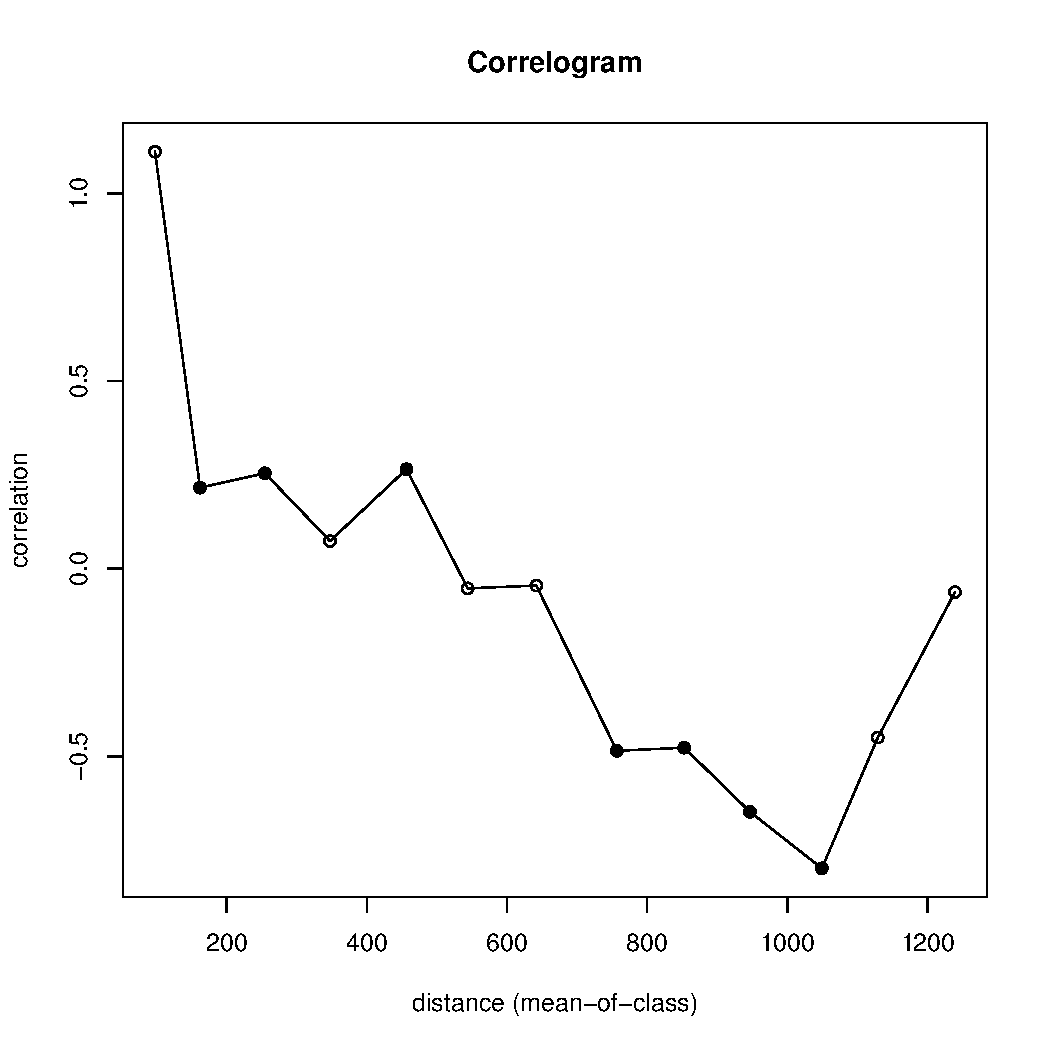
\includegraphics[width=65mm]{../Barenc_Sea/distribution_Moran/Pala_moran_N_Priapulus_caudatus_.pdf}
%	\end{center}
%	\end{minipage}
%
%	\hfil %Это пружинка отодвигающая рисунки друг от друга
%
%	\begin{minipage}[b]{.46\linewidth}
%Следующий рисунок - первый ряд справа %DUNGEON S_4 \ AB
%	\begin{center}
%		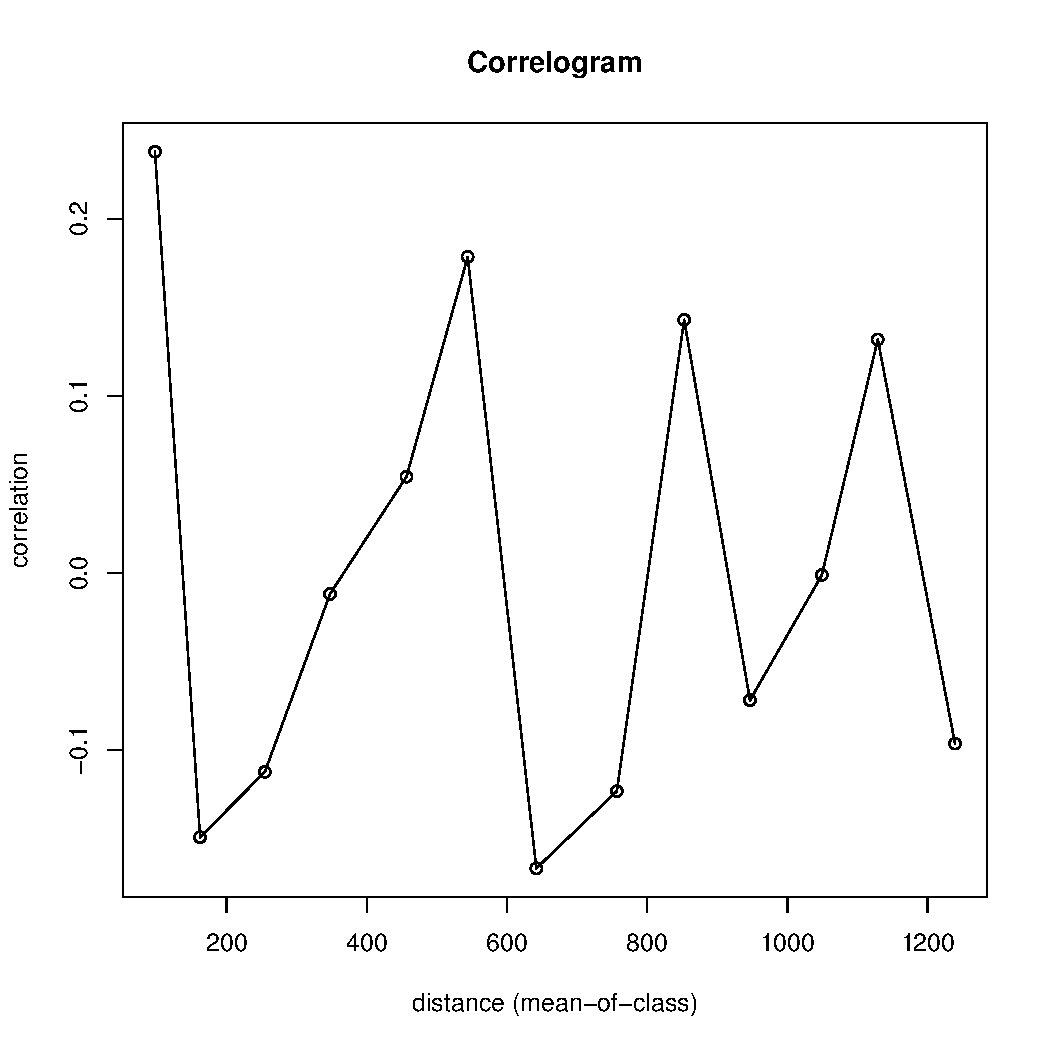
\includegraphics[width=65mm]{../Barenc_Sea/distribution_Moran/Pala_moran_B_Priapulus_caudatus_.pdf}
%	\end{center}
%	\end{minipage}

%\smallskip



%	\caption{Микрораспределение макробентоса на литорали Пала-губы (Продолжение)}
%	\label{ris:moransI_Pala}
	\begin{center}
	Рис. \ref{ris:moransI_Pala} (продолжение). Микрораспределение макробентоса на литорали Пала-губы.
	\end{center}

	\end{figure}



	\begin{figure}[h]

	\begin{minipage}[b]{.46\linewidth}
%Фигурка в первом ряду слева размер отведенный под весь этот объект \textendash 0.46 от ширины строки
%Параметр [b] означает, что выравнивание этих министраниц будет по нижнему краю
	\begin{center}
	{\small N~{\it Macoma balthica}}
		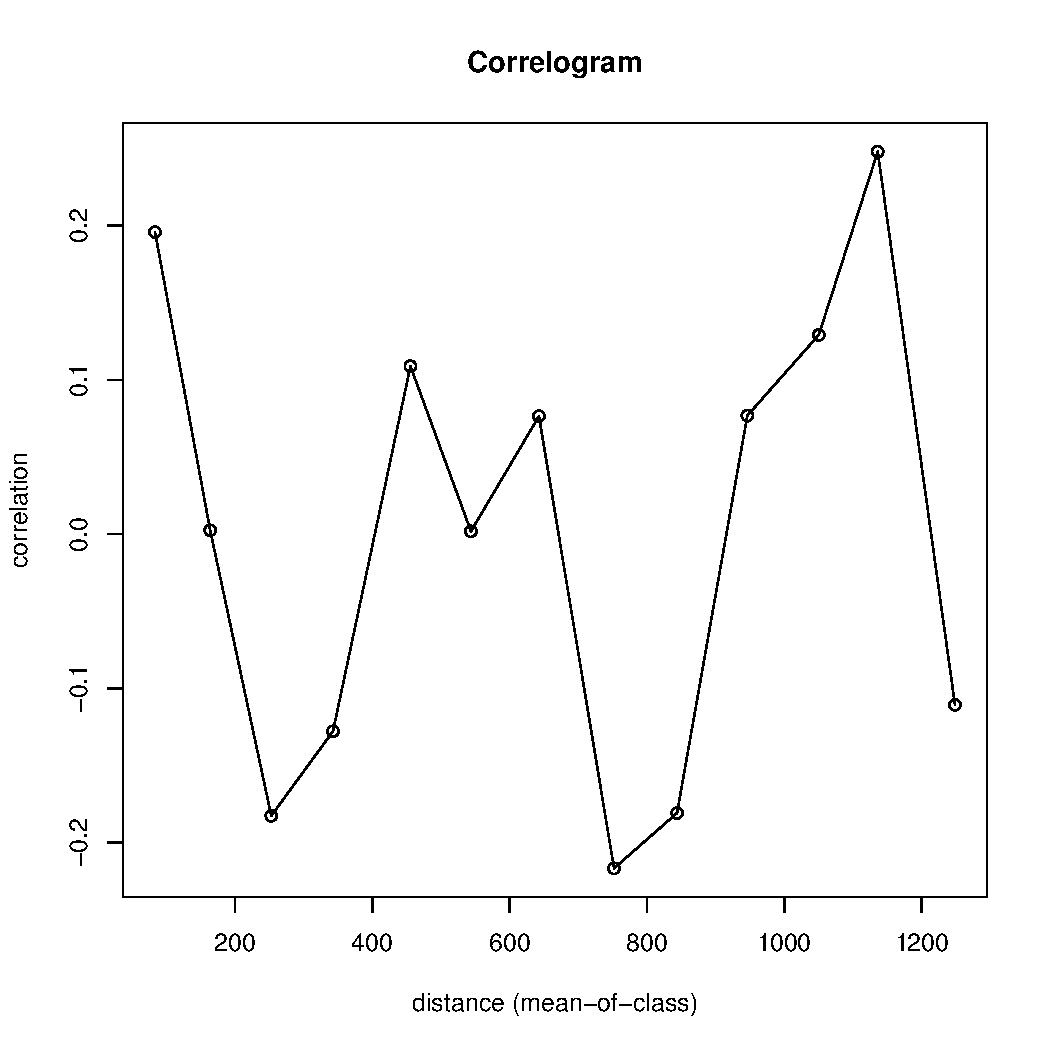
\includegraphics[width=65mm]{../Barenc_Sea/distribution_Moran/Plyazh07_moran_N_Macoma_balthica_.pdf}
	\end{center}
	\end{minipage}
%
	\hfil %Это пружинка отодвигающая рисунки друг от друга
%
	\begin{minipage}[b]{.46\linewidth}
%Следующий рисунок - первый ряд справа %DUNGEON S_4 \ AB
	\begin{center}
	{\small B~{\it Macoma balthica}}
		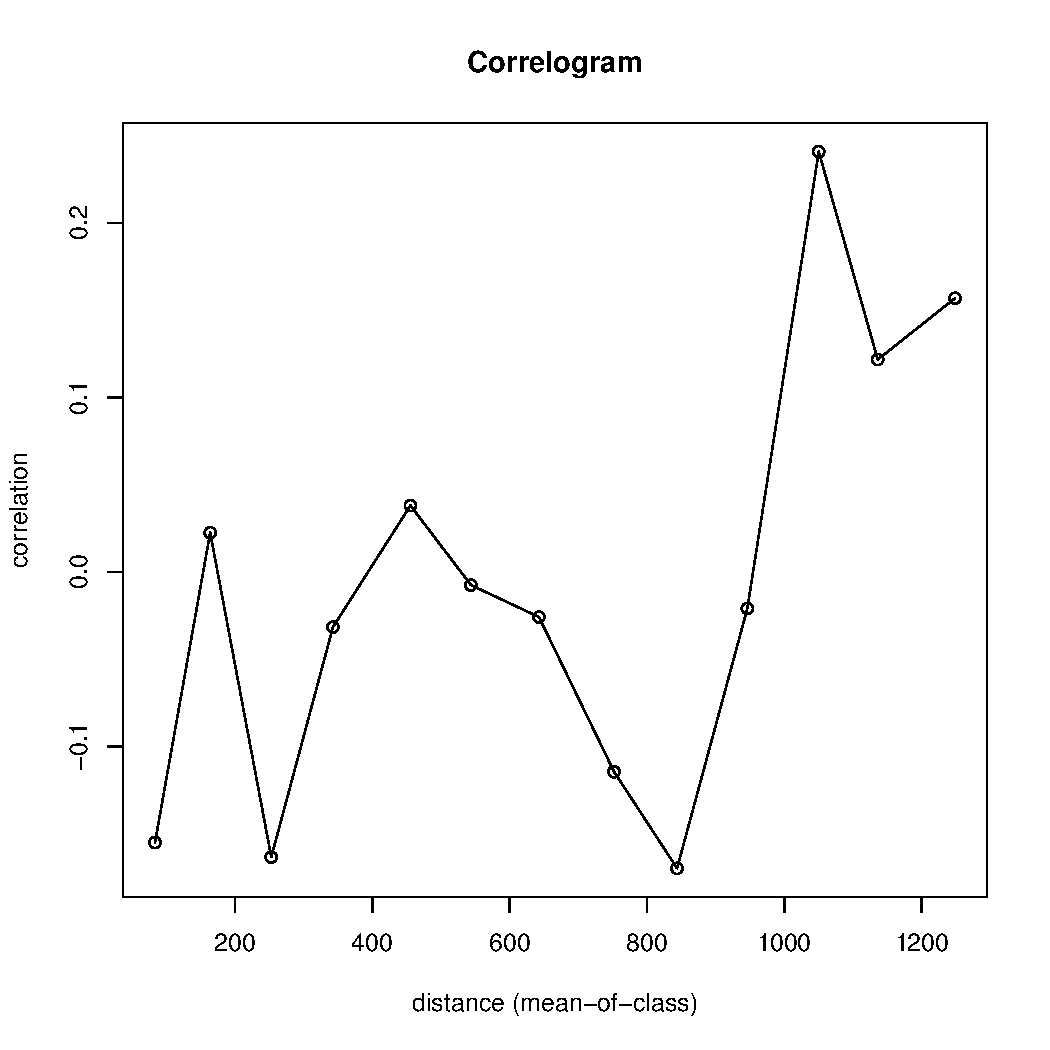
\includegraphics[width=65mm]{../Barenc_Sea/distribution_Moran/Plyazh07_moran_B_Macoma_balthica_.pdf}
	\end{center}
	\end{minipage}

	
	\begin{minipage}[b]{.46\linewidth}
	%Фигурка в первом ряду слева размер отведенный под весь этот объект \textendash 0.46 от ширины строки
	%Параметр [b] означает, что выравнивание этих министраниц будет по нижнему краю
	\begin{center}
	{\small N~{\it Cerastoderma edule}}
		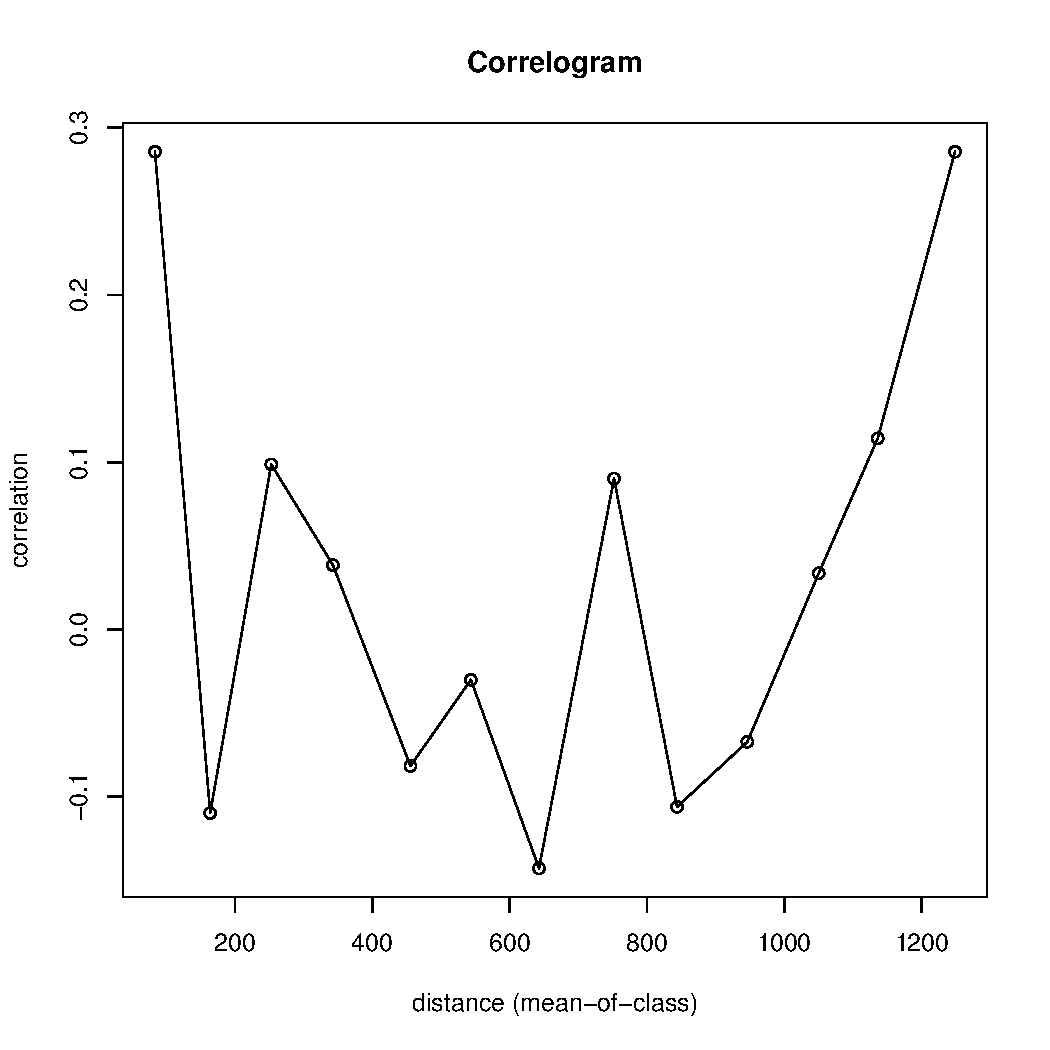
\includegraphics[width=65mm]{../Barenc_Sea/distribution_Moran/Plyazh07_moran_N_Cerastoderma_edule_.pdf}

	\end{center}
	\end{minipage}
	%
	\hfil %Это пружинка отодвигающая рисунки друг от друга
	%
	\begin{minipage}[b]{.46\linewidth}
%Следующий рисунок - первый ряд справа %DUNGEON S_4 \ AB
	\begin{center}
	{\small B~{\it Cerastoderma edule}}
		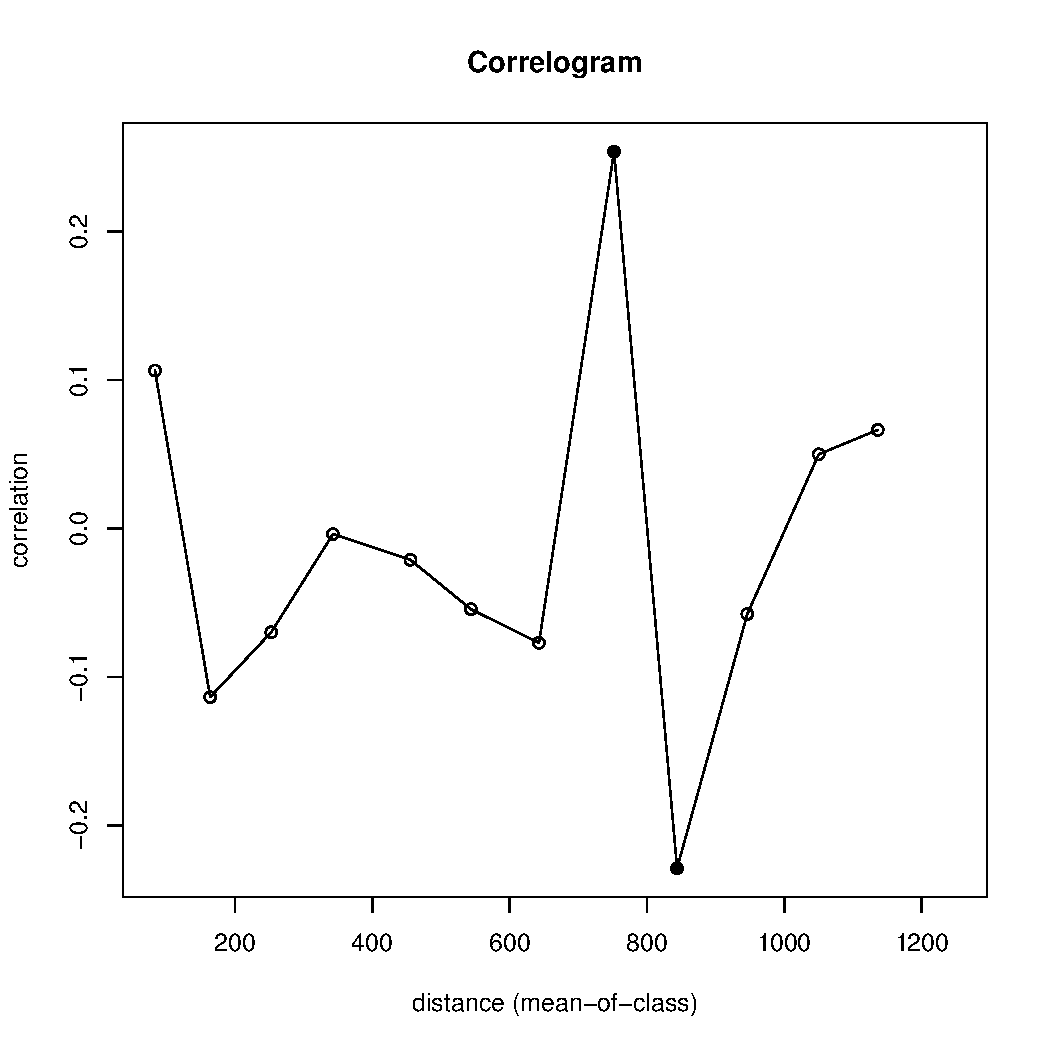
\includegraphics[width=65mm]{../Barenc_Sea/distribution_Moran/Plyazh07_moran_B_Cerastoderma_edule_.pdf}
	\end{center}
	\end{minipage}

%\smallskip



%\smallskip

	\begin{minipage}[b]{.46\linewidth}
%Фигурка в первом ряду слева размер отведенный под весь этот объект \textendash 0.46 от ширины строки
%Параметр [b] означает, что выравнивание этих министраниц будет по нижнему краю
	\begin{center}
	{\small N~{\it Mya arenaria}}
		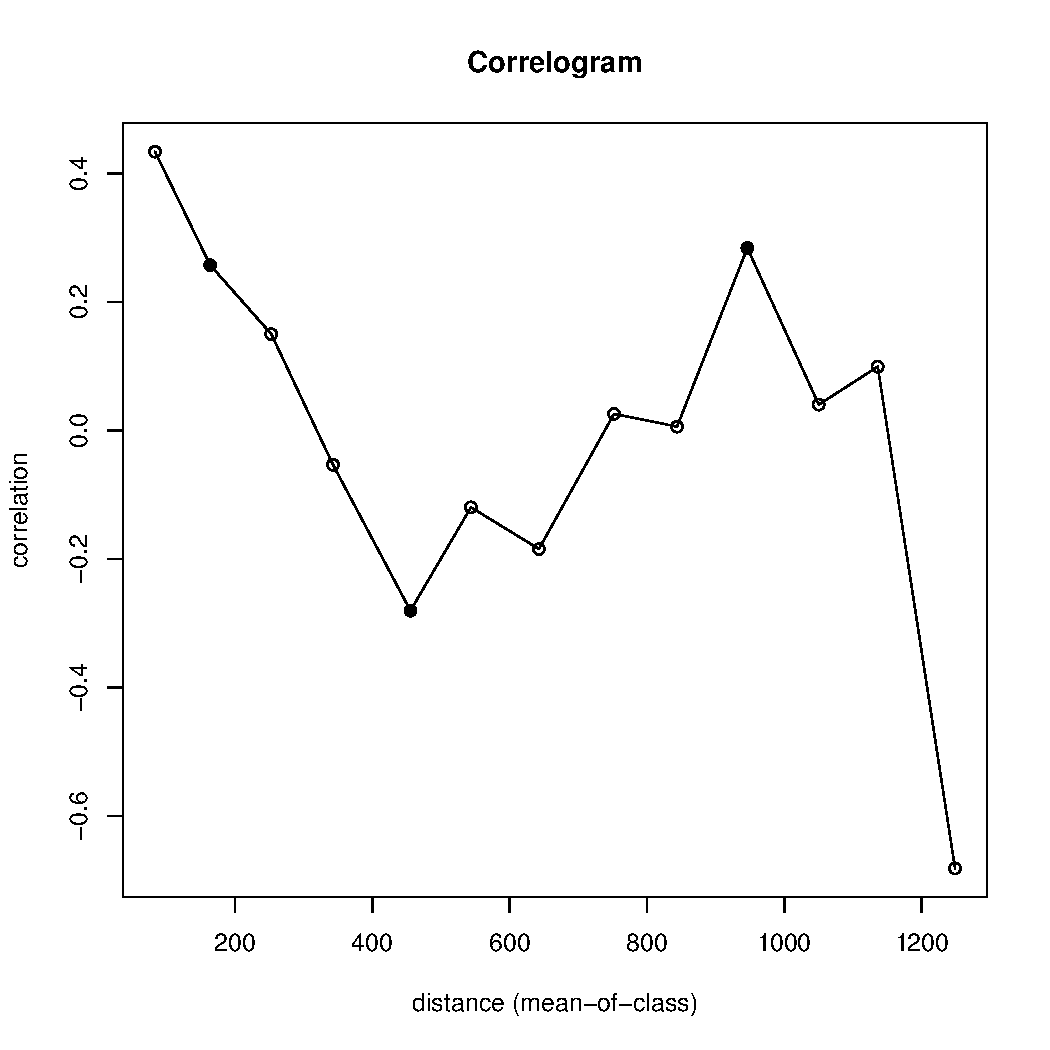
\includegraphics[width=65mm]{../Barenc_Sea/distribution_Moran/Plyazh07_moran_N_Mya_arenaria_.pdf}
	\end{center}
	\end{minipage}
%
	\hfil %Это пружинка отодвигающая рисунки друг от друга
%
	\begin{minipage}[b]{.46\linewidth}
%Следующий рисунок - первый ряд справа %DUNGEON S_4 \ AB
	\begin{center}
	{\small B~{\it Mya arenaria}}
		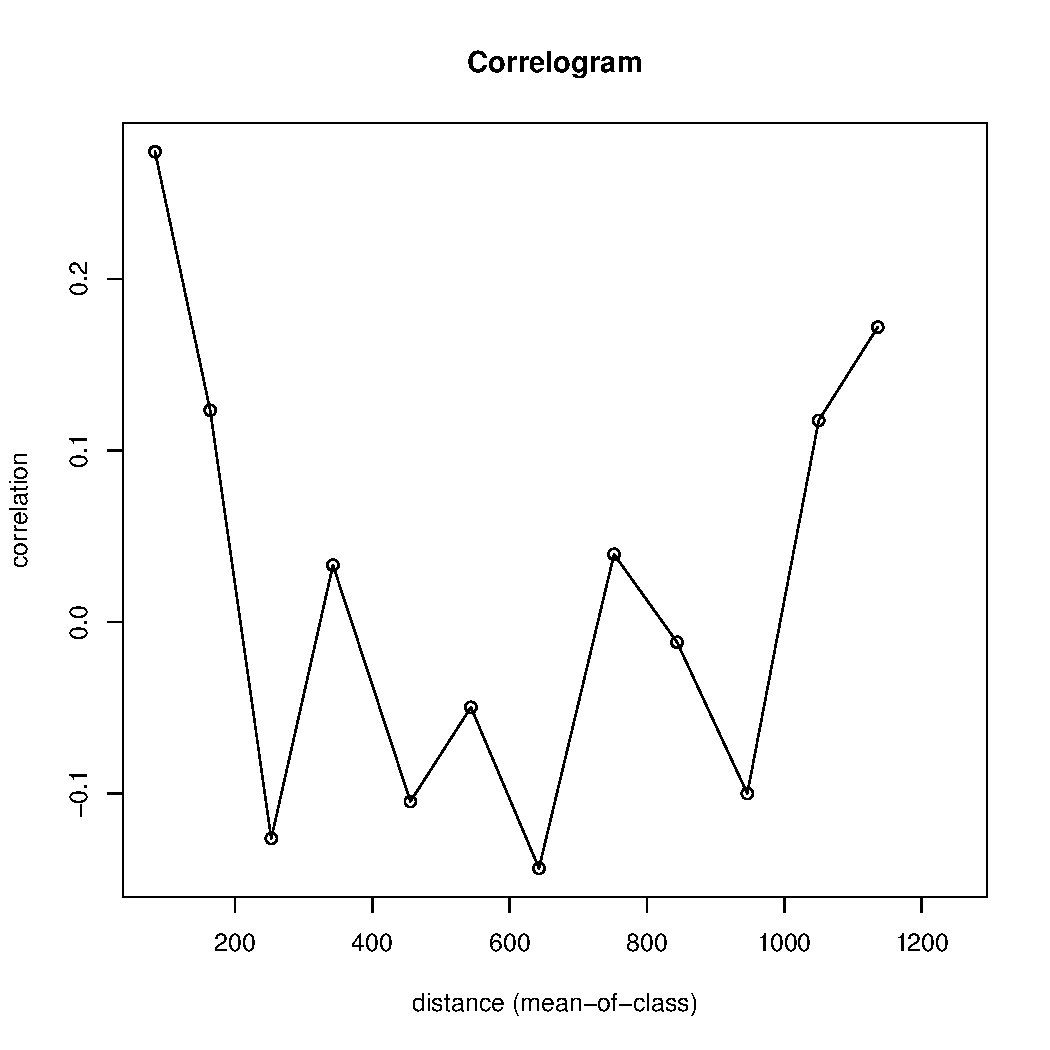
\includegraphics[width=65mm]{../Barenc_Sea/distribution_Moran/Plyazh07_moran_B_Mya_arenaria_.pdf}
	\end{center}
	\end{minipage}

%\smallskip


	\caption{Микрораспределение макробентоса на литорали Дальнего пляжа г.~Дальнезеленецкая в 2007 году.}
	\label{ris:moransI_Plyazh07_1}
	\end{figure}



	\begin{figure}[h]

	\begin{minipage}[b]{.46\linewidth}
%Фигурка в первом ряду слева размер отведенный под весь этот объект \textendash 0.46 от ширины строки
%Параметр [b] означает, что выравнивание этих министраниц будет по нижнему краю
	\begin{center}
	{\small N~{\it Mytilus edulis}}
		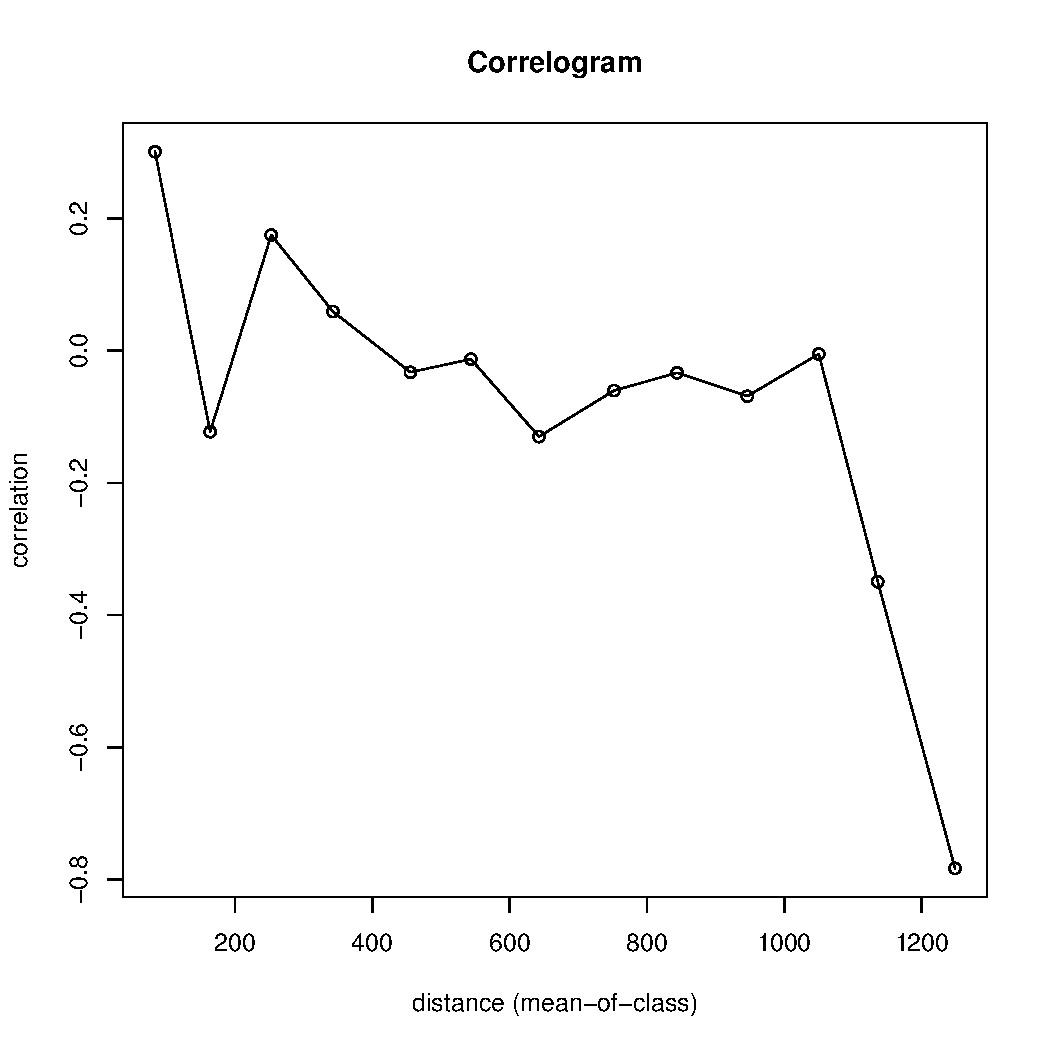
\includegraphics[width=65mm]{../Barenc_Sea/distribution_Moran/Plyazh07_moran_N_Mytilus_edulis_.pdf}
	\end{center}
	\end{minipage}
%
	\hfil %Это пружинка отодвигающая рисунки друг от друга
%
	\begin{minipage}[b]{.46\linewidth}
%Следующий рисунок - первый ряд справа %DUNGEON S_4 \ AB
	\begin{center}
	{\small B~{\it Mytilus edulis}}
		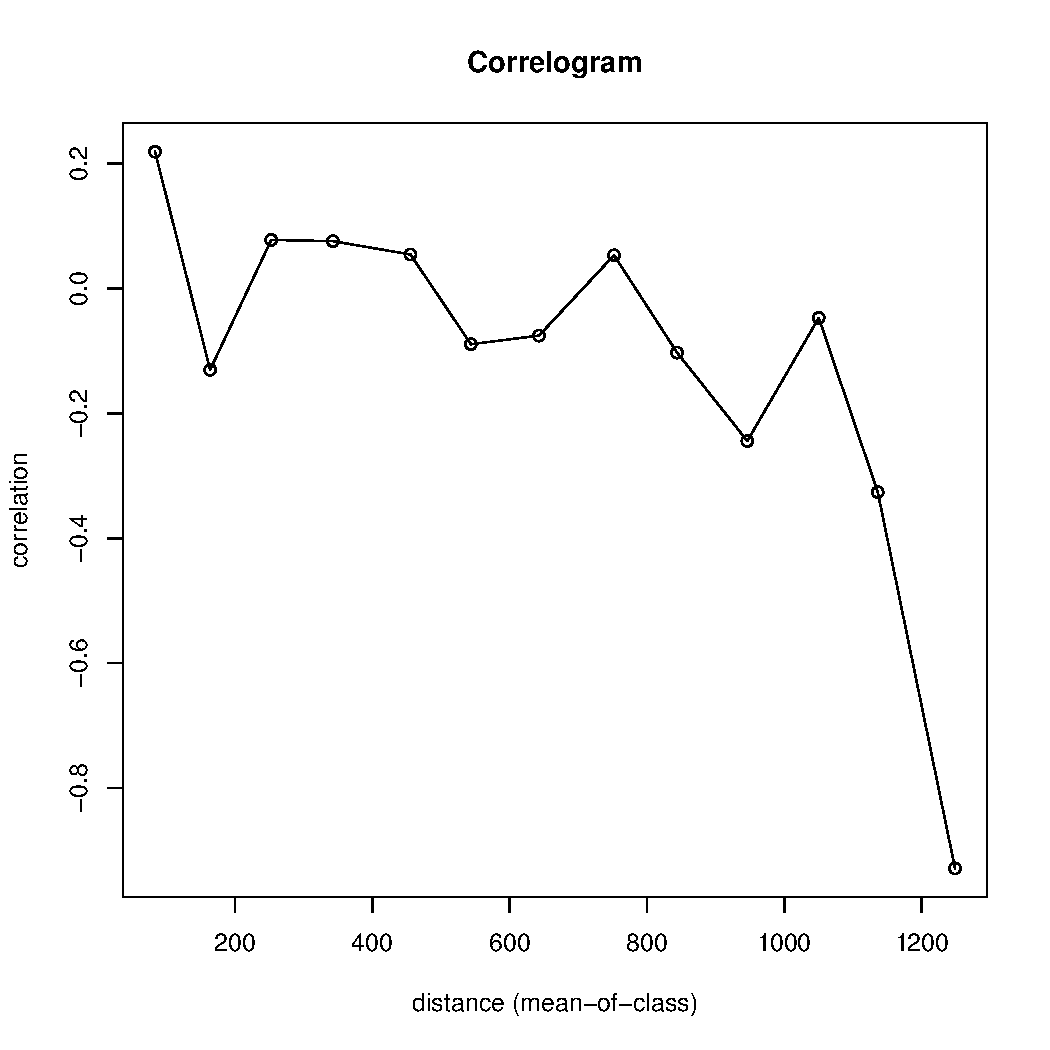
\includegraphics[width=65mm]{../Barenc_Sea/distribution_Moran/Plyazh07_moran_B_Mytilus_edulis_.pdf}
	\end{center}
	\end{minipage}

	
	\begin{minipage}[b]{.46\linewidth}
	%Фигурка в первом ряду слева размер отведенный под весь этот объект \textendash 0.46 от ширины строки
	%Параметр [b] означает, что выравнивание этих министраниц будет по нижнему краю
	\begin{center}
	{\small N~{\it Pseudolibrotus littoralis}}
	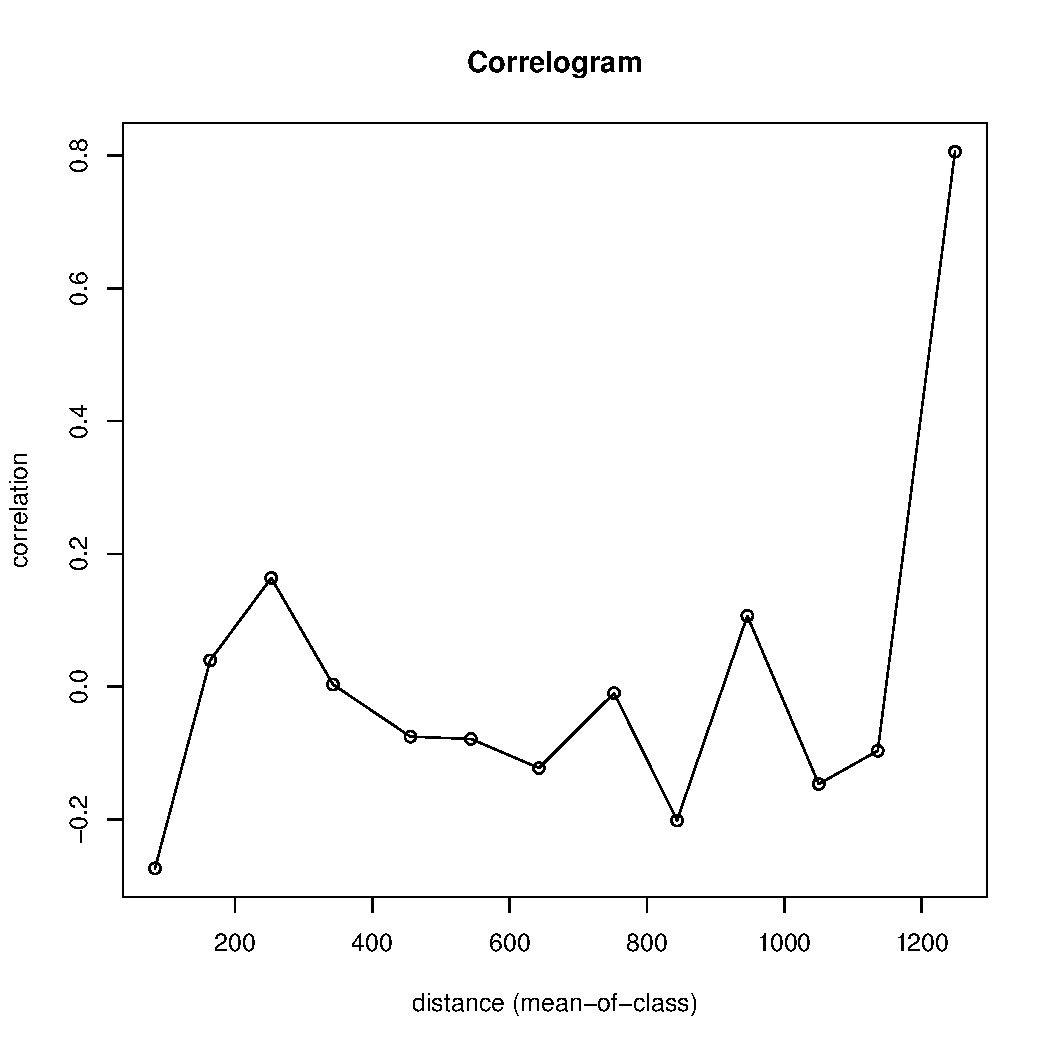
\includegraphics[width=65mm]{../Barenc_Sea/distribution_Moran/Plyazh07_moran_N_Pseudolibrotus_littoralis_.pdf}

	\end{center}
	\end{minipage}
	%
	\hfil %Это пружинка отодвигающая рисунки друг от друга
	%
	\begin{minipage}[b]{.46\linewidth}
%Следующий рисунок - первый ряд справа %DUNGEON S_4 \ AB
	\begin{center}
	{\small B~{\it Pseudolibrotus littoralis}}
		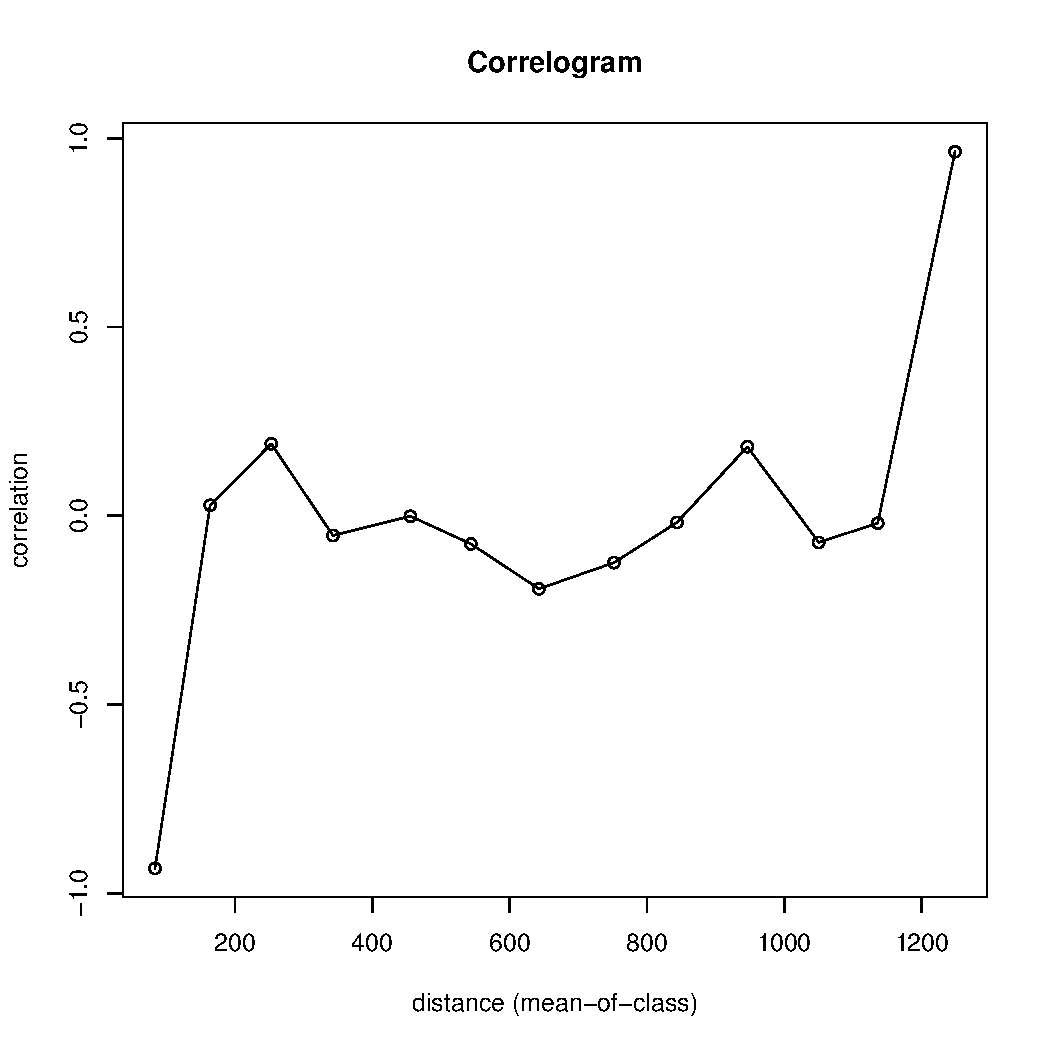
\includegraphics[width=65mm]{../Barenc_Sea/distribution_Moran/Plyazh07_moran_B_Pseudolibrotus_littoralis_.pdf}
	\end{center}
	\end{minipage}

%\smallskip



%\smallskip

	\begin{minipage}[b]{.46\linewidth}
%Фигурка в первом ряду слева размер отведенный под весь этот объект \textendash 0.46 от ширины строки
%Параметр [b] означает, что выравнивание этих министраниц будет по нижнему краю
	\begin{center}
	{\small N~{\it Gammarus sp.}}
		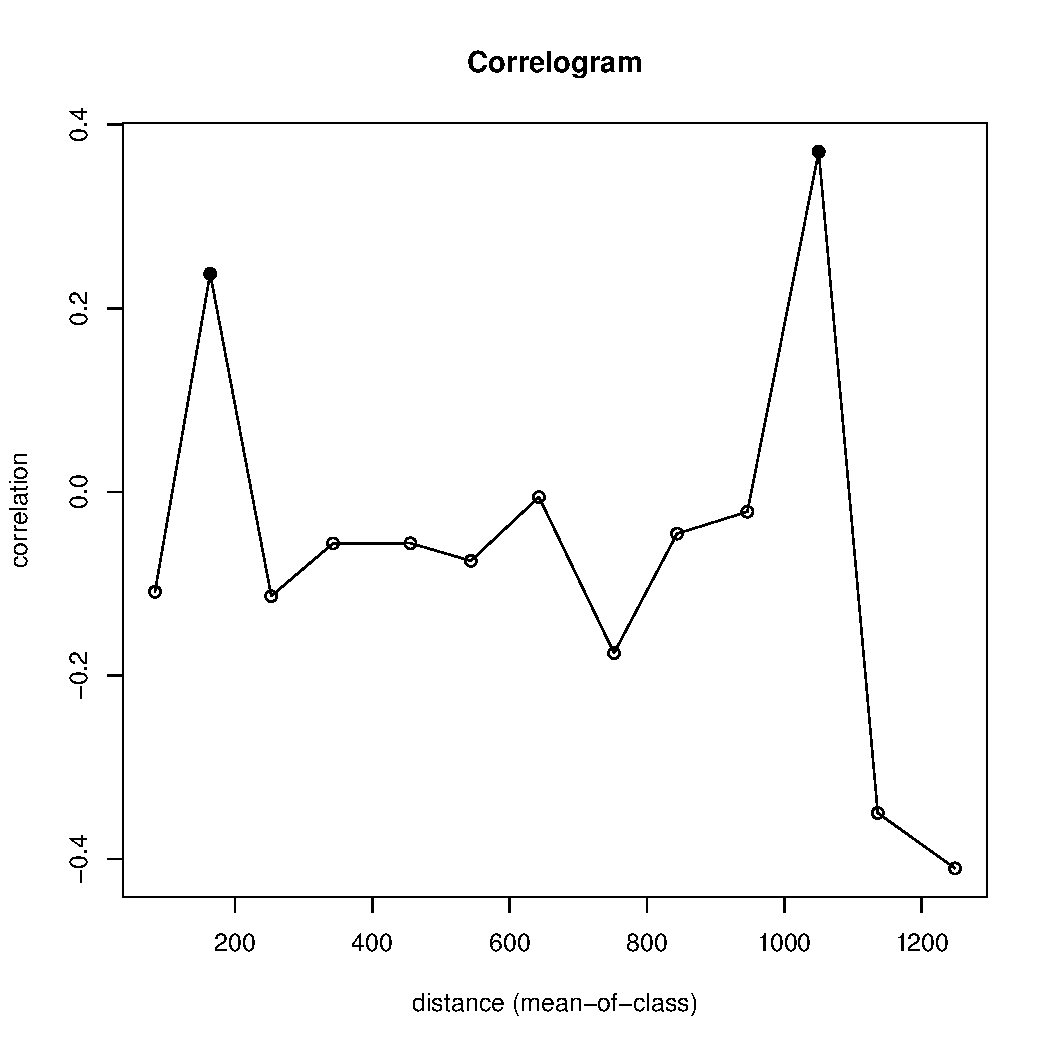
\includegraphics[width=65mm]{../Barenc_Sea/distribution_Moran/Plyazh07_moran_N_Gammarus_sp_.pdf}
	\end{center}
	\end{minipage}
%
%	\hfil %Это пружинка отодвигающая рисунки друг от друга
%
%	\begin{minipage}[b]{.46\linewidth}
%Следующий рисунок - первый ряд справа %DUNGEON S_4 \ AB
%	\begin{center}
%		\includegraphics[width=65mm]{../Barenc_Sea/distribution_Moran/Plyazh07_moran_B_Mya_arenaria__.pdf}
%	\end{center}
%	\end{minipage}

%\smallskip


%	\caption{Микрораспределение макробентоса на литорали Дальнего пляжа г.~Дальнезеленецкая в 2007 году (продолжение).}
%	\label{ris:moransI_Plyazh07_1}
%	\end{figure}
	\begin{center}
	Рис. \ref{ris:moransI_Plyazh07_1} (продолжение). Микрораспределение макробентоса на литорали Дальнего пляжа г.~Дальнезеленецкая в 2007 году.
	\end{center}

\end{figure}



	\begin{figure}[h]

	\begin{minipage}[b]{.46\linewidth}
%Фигурка в первом ряду слева размер отведенный под весь этот объект \textendash 0.46 от ширины строки
%Параметр [b] означает, что выравнивание этих министраниц будет по нижнему краю
	\begin{center}
	{\small N~{\it Macoma balthica}}
		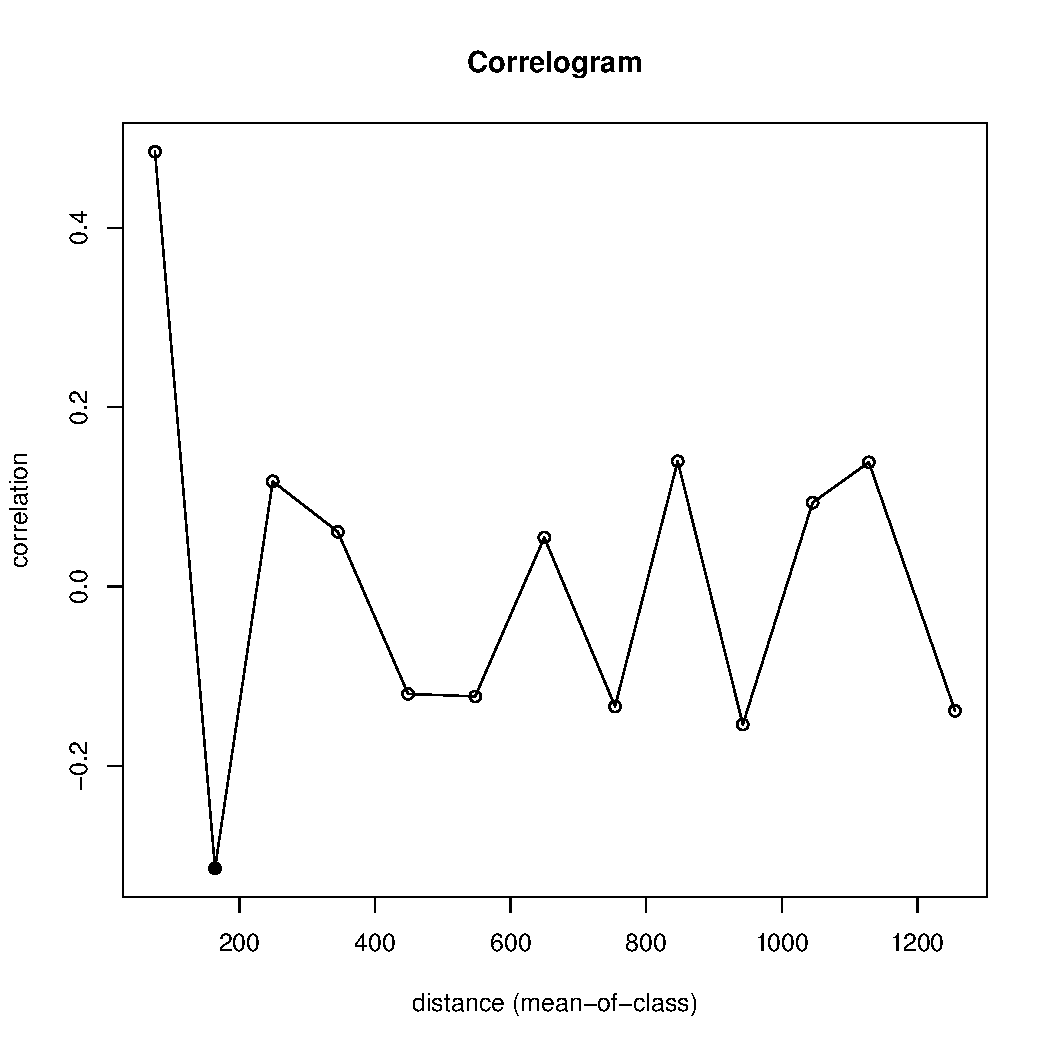
\includegraphics[width=65mm]{../Barenc_Sea/distribution_Moran/Plyazh081_moran_N_Macoma_balthica_.pdf}
	\end{center}
	\end{minipage}
%
	\hfil %Это пружинка отодвигающая рисунки друг от друга
%
	\begin{minipage}[b]{.46\linewidth}
%Следующий рисунок - первый ряд справа %DUNGEON S_4 \ AB
	\begin{center}
	{\small B~{\it Macoma balthica}}
		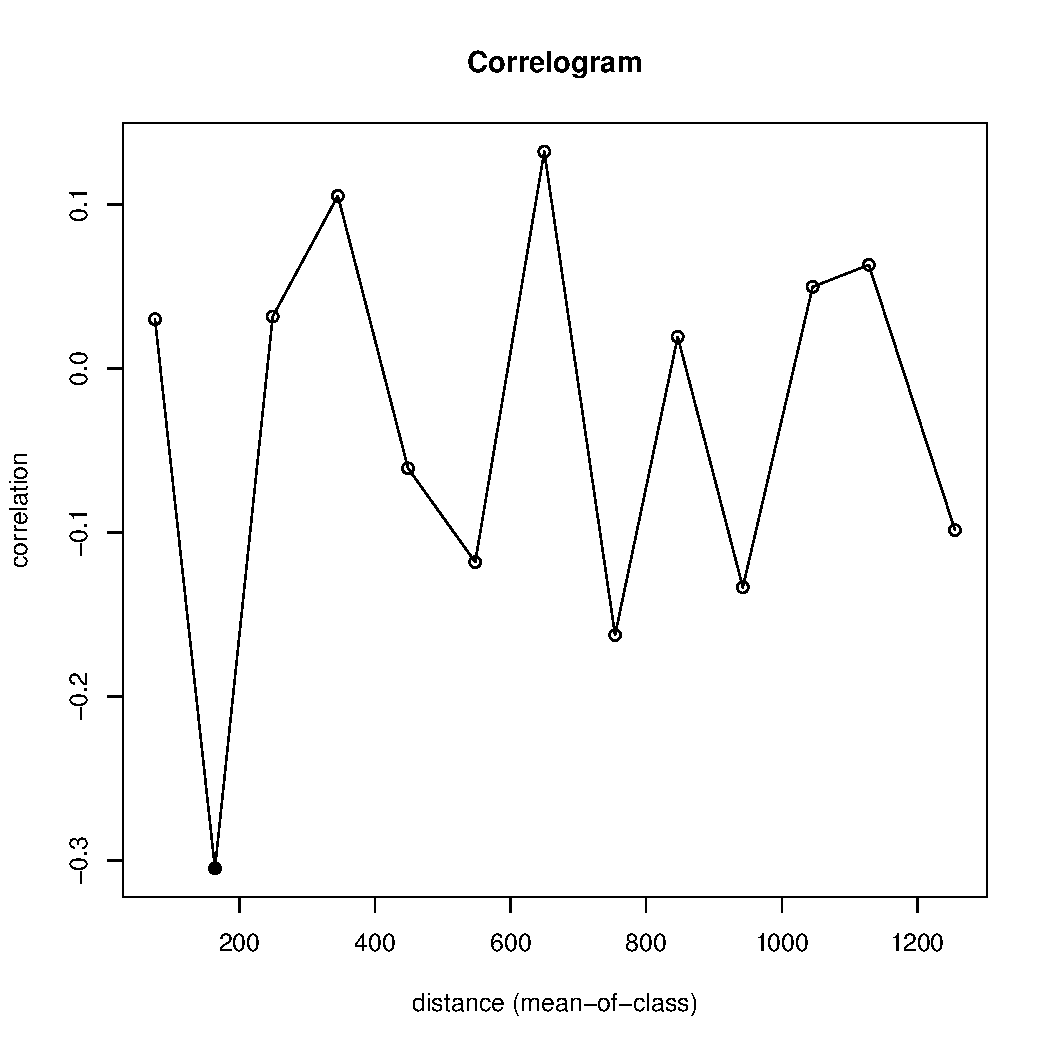
\includegraphics[width=65mm]{../Barenc_Sea/distribution_Moran/Plyazh081_moran_B_Macoma_balthica_.pdf}
	\end{center}
	\end{minipage}

	
	\begin{minipage}[b]{.46\linewidth}
	%Фигурка в первом ряду слева размер отведенный под весь этот объект \textendash 0.46 от ширины строки
	%Параметр [b] означает, что выравнивание этих министраниц будет по нижнему краю
	\begin{center}
	{\small N~{\it Cerastoderma edule}}
		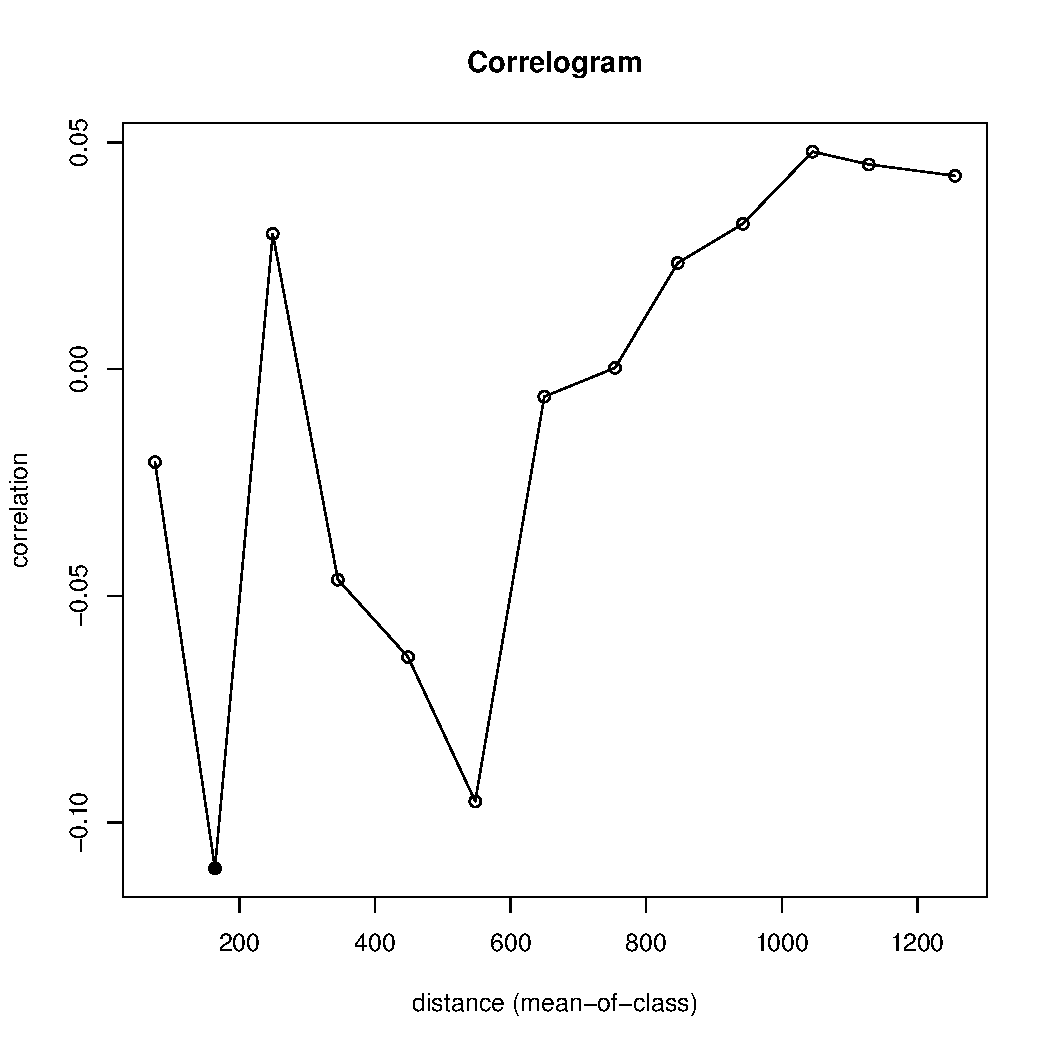
\includegraphics[width=65mm]{../Barenc_Sea/distribution_Moran/Plyazh081_moran_B_Cerastoderma_edule_.pdf}

	\end{center}
	\end{minipage}
	%
	\hfil %Это пружинка отодвигающая рисунки друг от друга
	%
	\begin{minipage}[b]{.46\linewidth}
%Следующий рисунок - первый ряд справа %DUNGEON S_4 \ AB
	\begin{center}
	{\small B~{\it Cerastoderma edule}}
		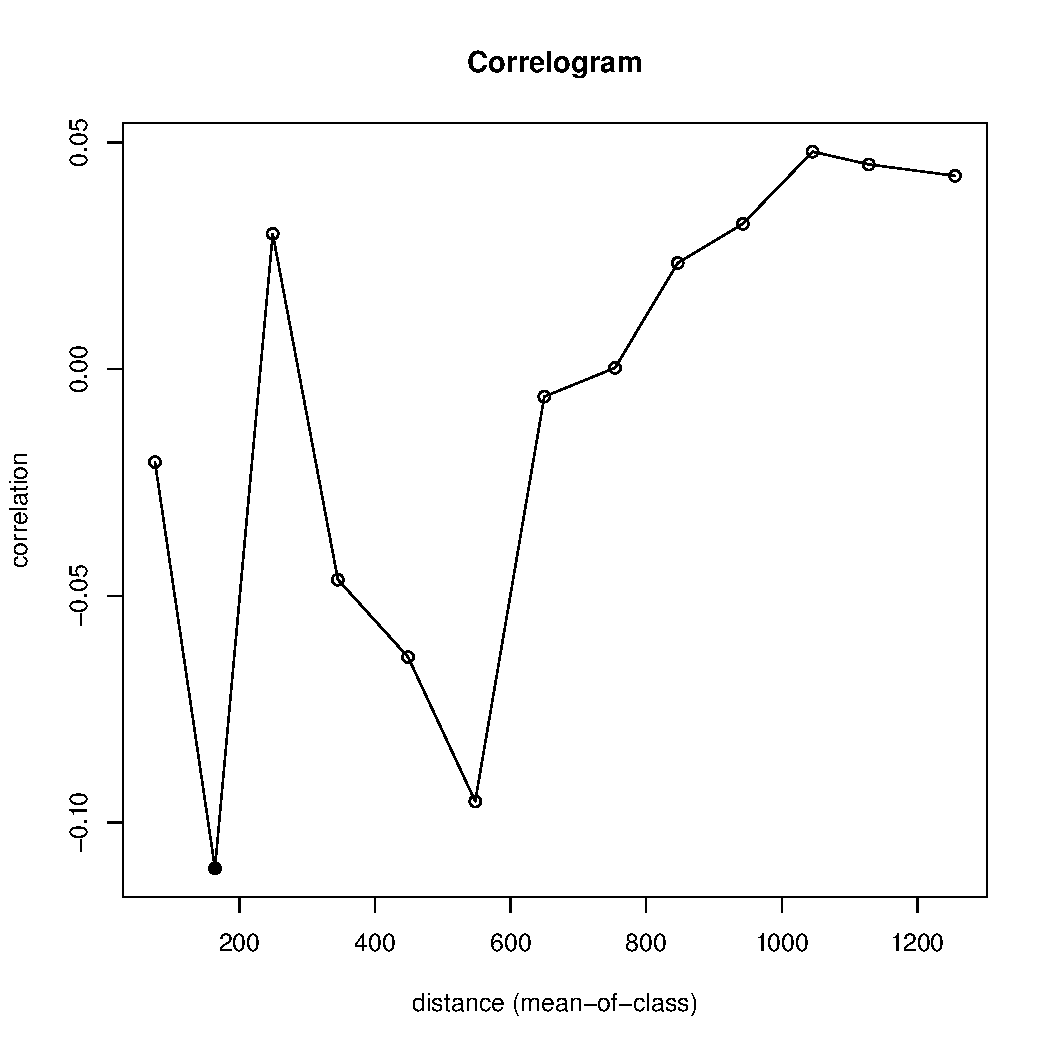
\includegraphics[width=65mm]{../Barenc_Sea/distribution_Moran/Plyazh081_moran_B_Cerastoderma_edule_.pdf}
	\end{center}
	\end{minipage}

%\smallskip



%\smallskip

	\begin{minipage}[b]{.46\linewidth}
%Фигурка в первом ряду слева размер отведенный под весь этот объект \textendash 0.46 от ширины строки
%Параметр [b] означает, что выравнивание этих министраниц будет по нижнему краю
	\begin{center}
	{\small N~{\it Mya arenaria}}
		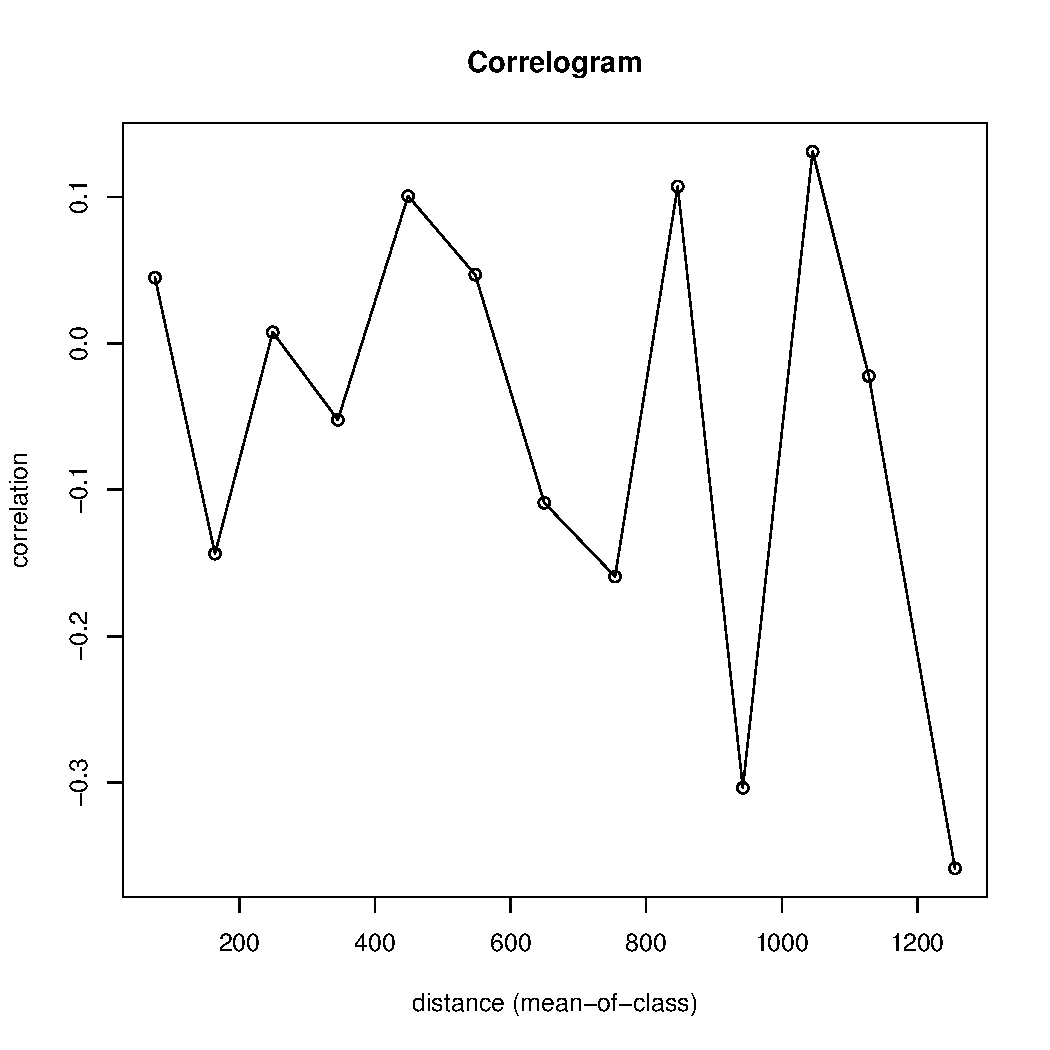
\includegraphics[width=65mm]{../Barenc_Sea/distribution_Moran/Plyazh081_moran_N_Mya_arenaria_.pdf}
	\end{center}
	\end{minipage}
%
	\hfil %Это пружинка отодвигающая рисунки друг от друга
%
	\begin{minipage}[b]{.46\linewidth}
%Следующий рисунок - первый ряд справа %DUNGEON S_4 \ AB
	\begin{center}
	{\small B~{\it Mya arenaria}}
		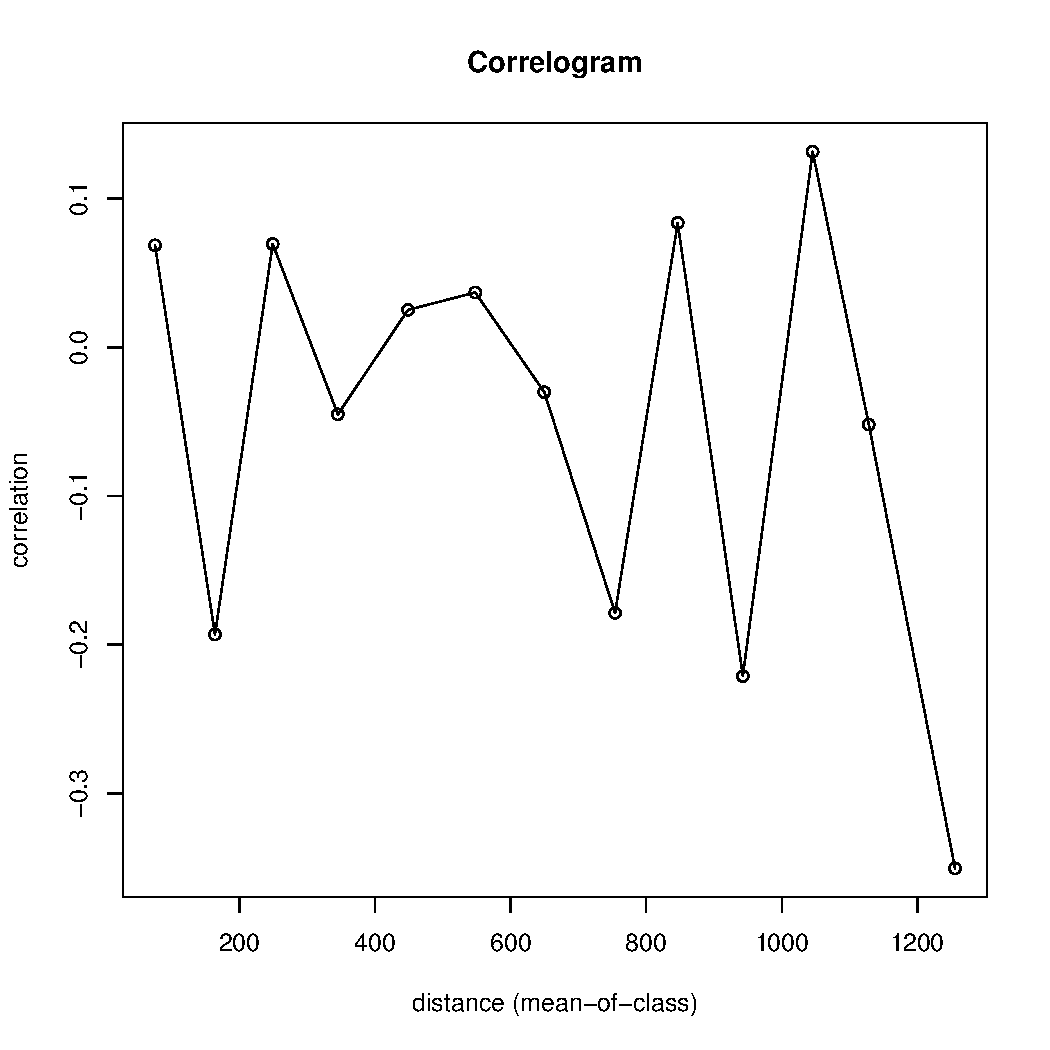
\includegraphics[width=65mm]{../Barenc_Sea/distribution_Moran/Plyazh081_moran_B_Mya_arenaria_.pdf}
	\end{center}
	\end{minipage}

%\smallskip


	\caption{Микрораспределение макробентоса на 1 участке на литорали Дальнего пляжа г.~Дальнезеленецкая в 2008 году.}
	\label{ris:moransI_Plyazh081_1}
	\end{figure}



	\begin{figure}[h]

	\begin{minipage}[b]{.46\linewidth}
%Фигурка в первом ряду слева размер отведенный под весь этот объект \textendash 0.46 от ширины строки
%Параметр [b] означает, что выравнивание этих министраниц будет по нижнему краю
	\begin{center}
	{\small N~{\it Mytilus edulis}}
		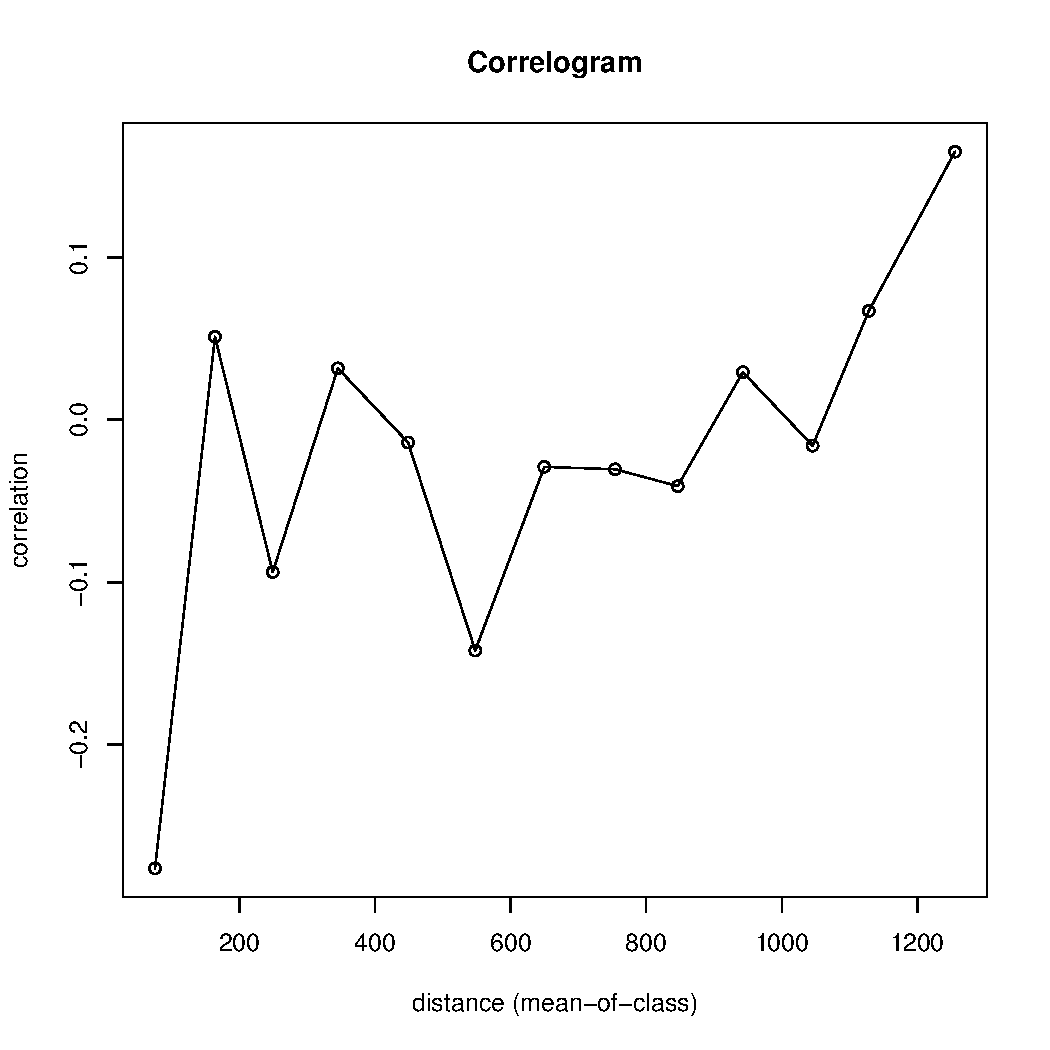
\includegraphics[width=65mm]{../Barenc_Sea/distribution_Moran/Plyazh081_moran_N_Mytilus_edulis_.pdf}
	\end{center}
	\end{minipage}
%
	\hfil %Это пружинка отодвигающая рисунки друг от друга
%
	\begin{minipage}[b]{.46\linewidth}
%Следующий рисунок - первый ряд справа %DUNGEON S_4 \ AB
	\begin{center}
	{\small B~{\it Mytilus edulis}}
		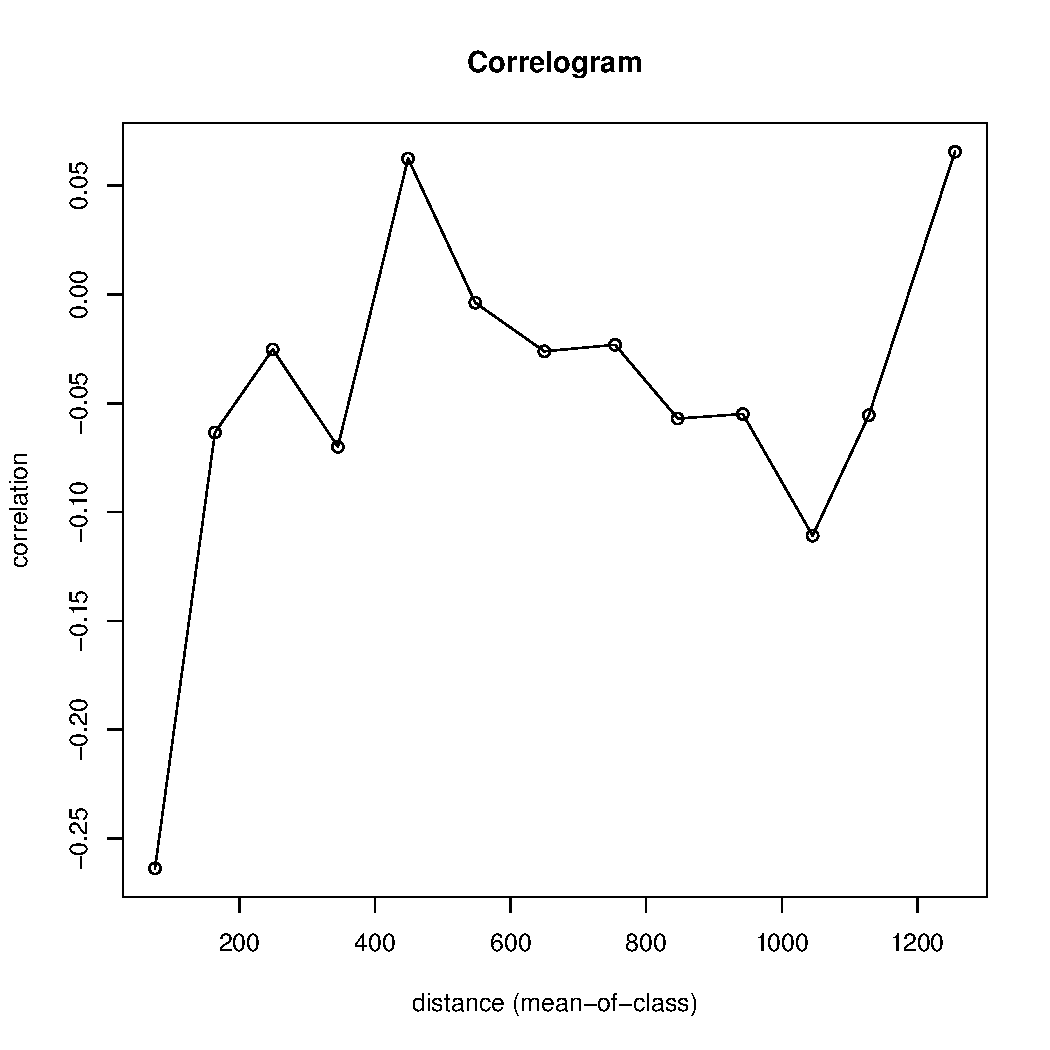
\includegraphics[width=65mm]{../Barenc_Sea/distribution_Moran/Plyazh081_moran_B_Mytilus_edulis_.pdf}
	\end{center}
	\end{minipage}

	
	\begin{minipage}[b]{.46\linewidth}
	%Фигурка в первом ряду слева размер отведенный под весь этот объект \textendash 0.46 от ширины строки
	%Параметр [b] означает, что выравнивание этих министраниц будет по нижнему краю
	\begin{center}
	{\small N~{\it Pseudolibrotus littoralis}}
	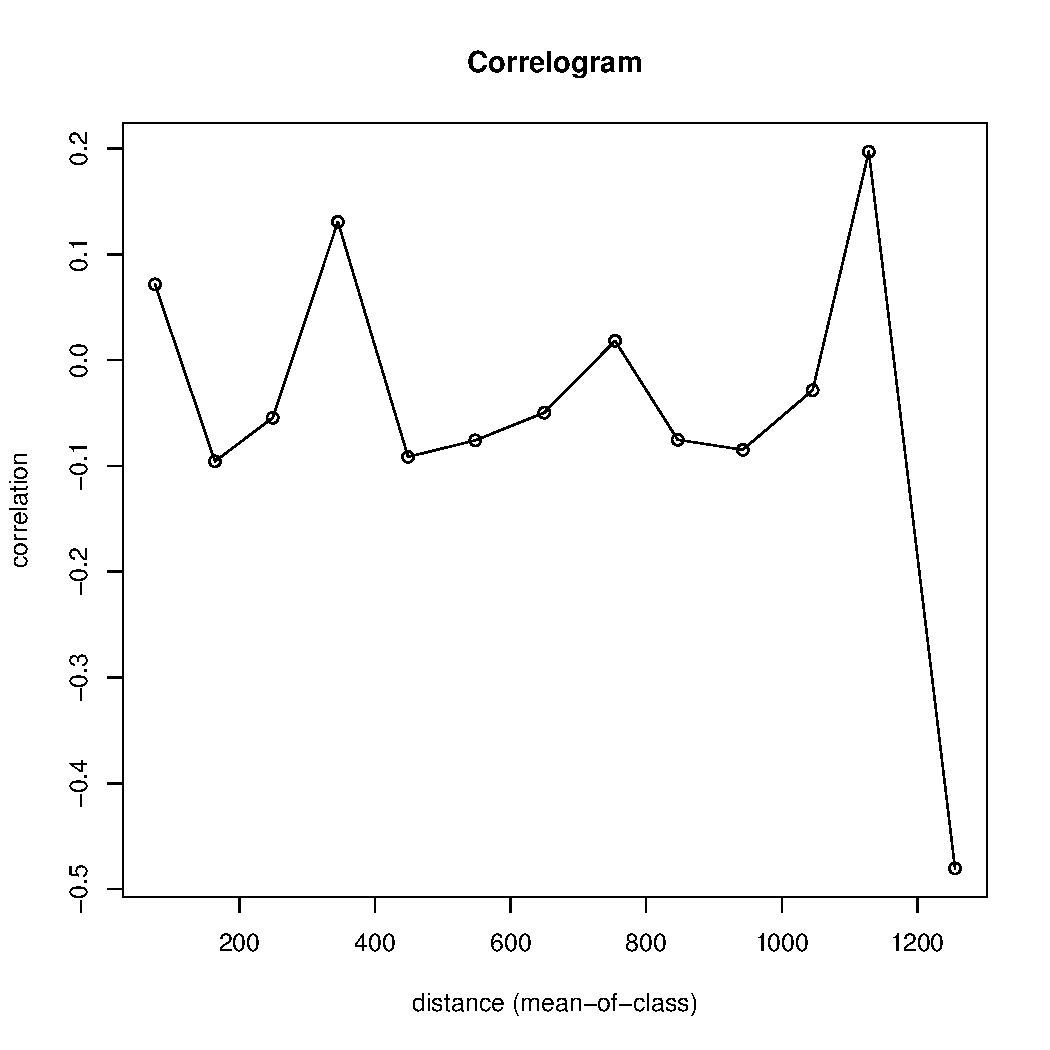
\includegraphics[width=65mm]{../Barenc_Sea/distribution_Moran/Plyazh081_moran_N_Pseudolibrotus_littoralis_.pdf}

	\end{center}
	\end{minipage}
	%
	\hfil %Это пружинка отодвигающая рисунки друг от друга
	%
	\begin{minipage}[b]{.46\linewidth}
%Следующий рисунок - первый ряд справа %DUNGEON S_4 \ AB
	\begin{center}
	{\small B~{\it Pseudolibrotus littoralis}}
		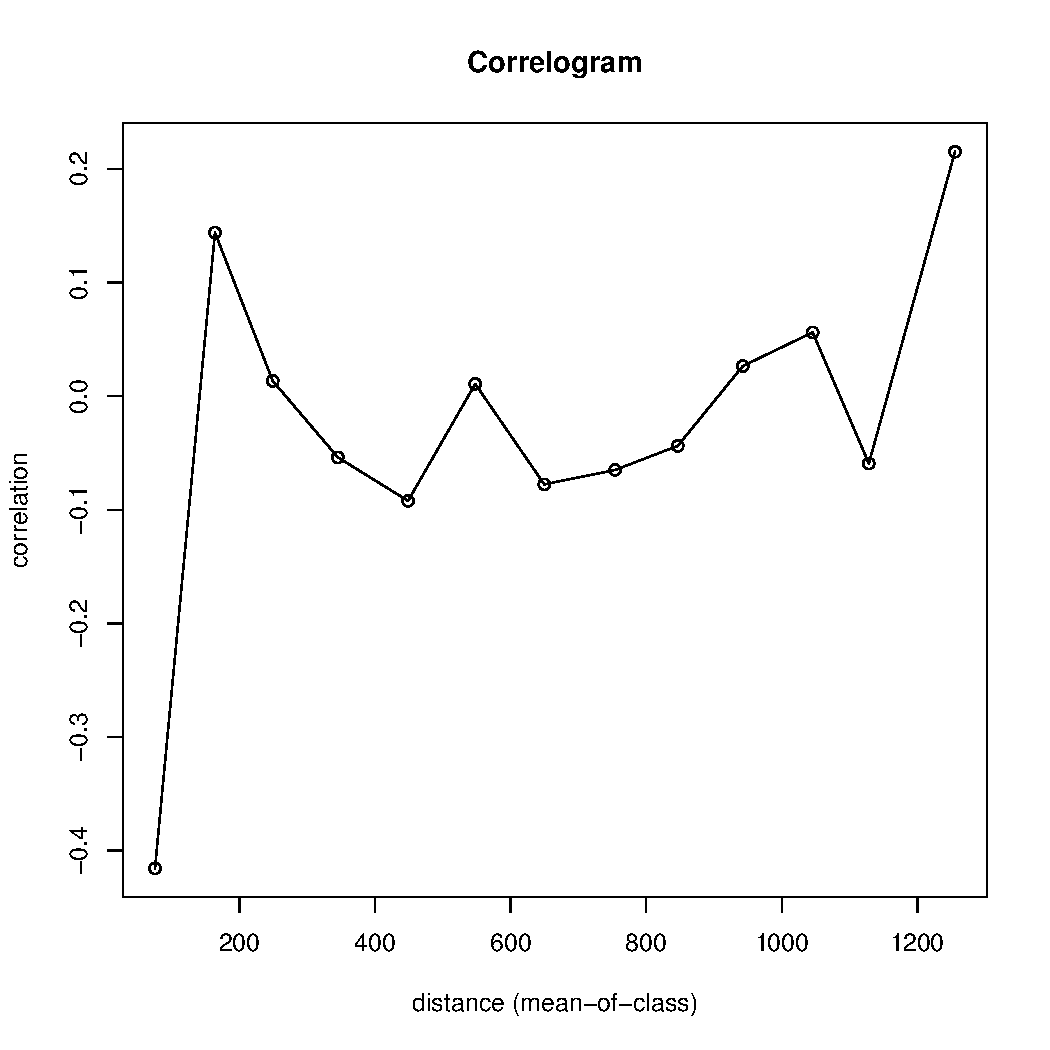
\includegraphics[width=65mm]{../Barenc_Sea/distribution_Moran/Plyazh081_moran_B_Pseudolibrotus_littoralis_.pdf}
	\end{center}
	\end{minipage}

%\smallskip



%\smallskip

	\begin{minipage}[b]{.46\linewidth}
%Фигурка в первом ряду слева размер отведенный под весь этот объект \textendash 0.46 от ширины строки
%Параметр [b] означает, что выравнивание этих министраниц будет по нижнему краю
	\begin{center}
	{\small N~{\it Gammarus sp.}}
		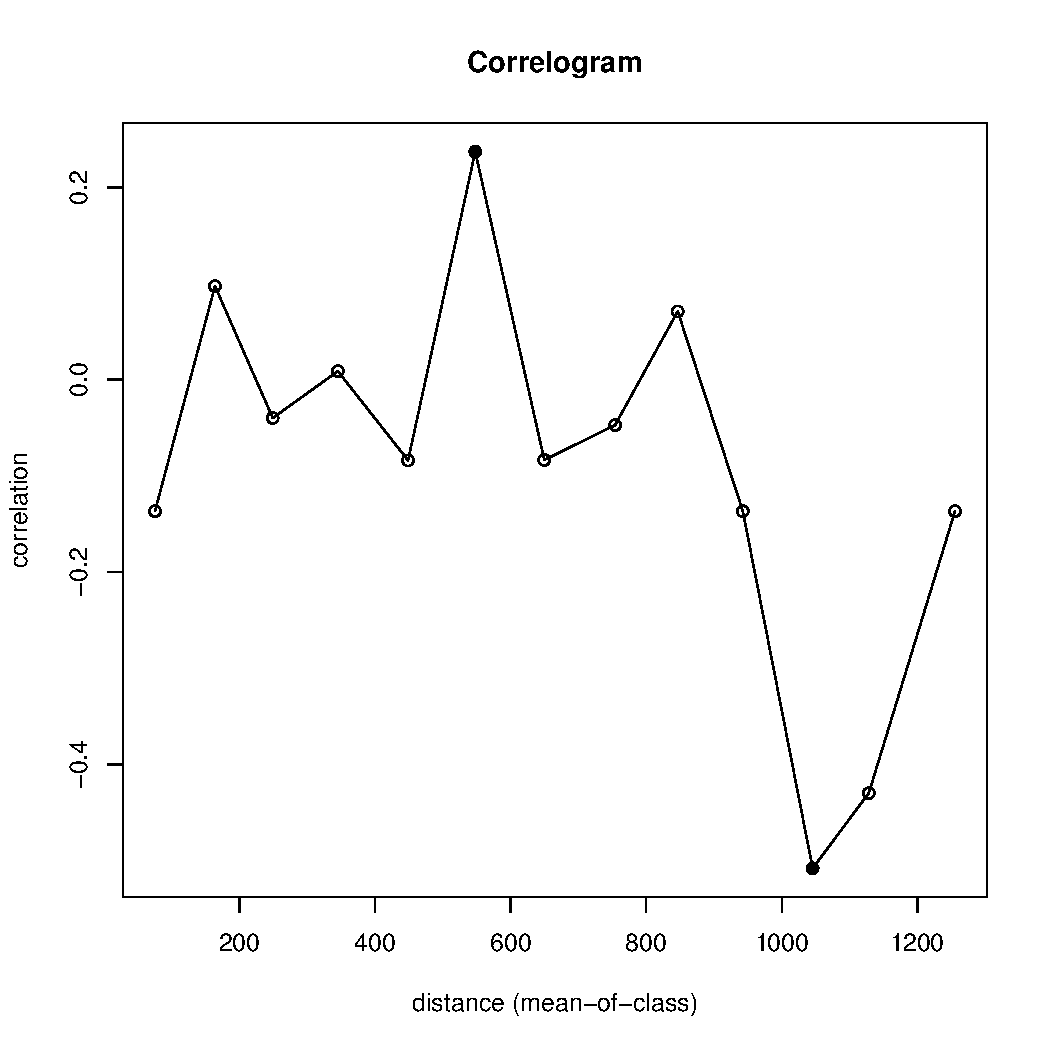
\includegraphics[width=65mm]{../Barenc_Sea/distribution_Moran/Plyazh081_moran_N_Gammarus_sp_.pdf}
	\end{center}
	\end{minipage}
%
	\hfil %Это пружинка отодвигающая рисунки друг от друга
%
	\begin{minipage}[b]{.46\linewidth}
%Следующий рисунок - первый ряд справа %DUNGEON S_4 \ AB
	\begin{center}
	{\small B~{\it Gammarus sp.}}
		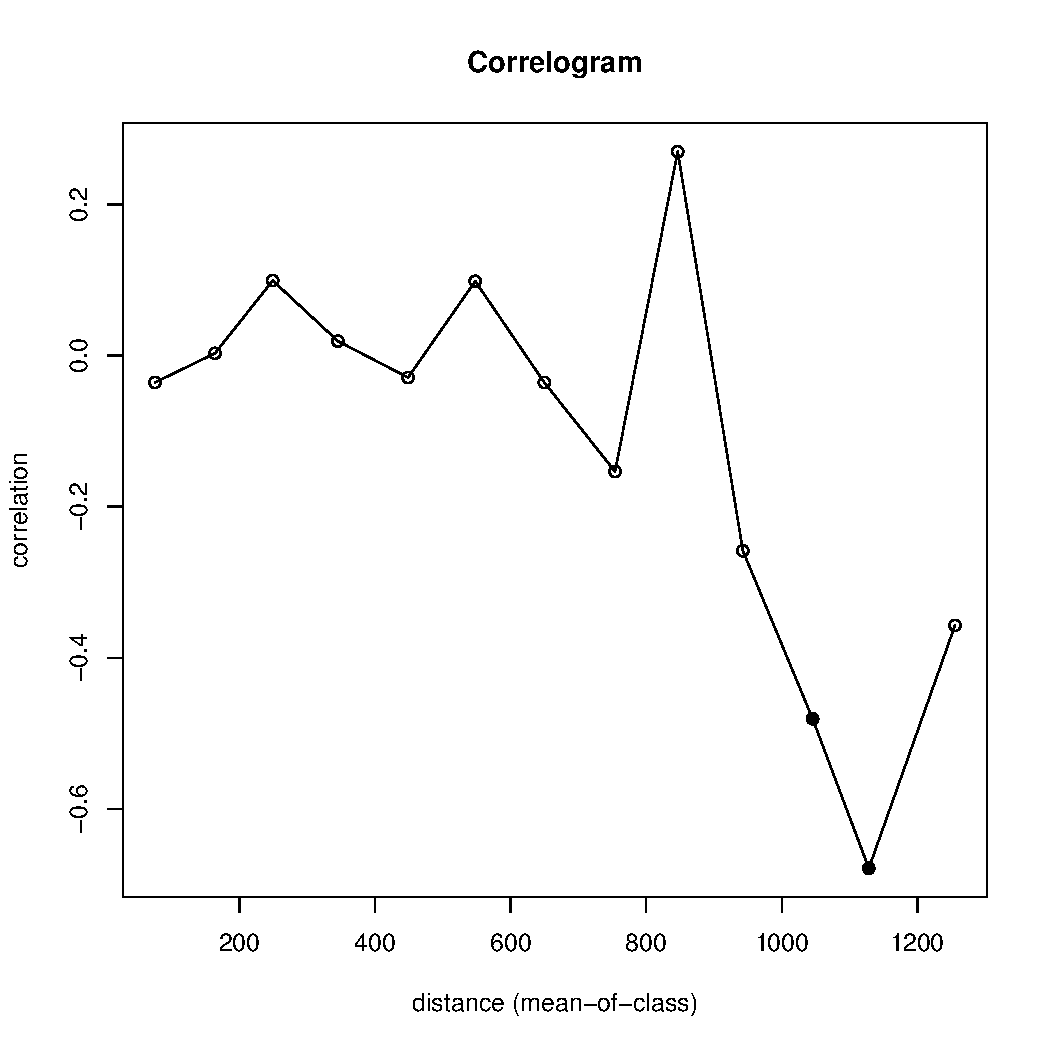
\includegraphics[width=65mm]{../Barenc_Sea/distribution_Moran/Plyazh081_moran_B_Gammarus_sp_.pdf}
	\end{center}
	\end{minipage}

%\smallskip


%	\caption{Микрораспределение макробентоса на литорали Дальнего пляжа г.~Дальнезеленецкая в 2007 году (продолжение).}
%	\label{ris:moransI_Plyazh081_1}
%	\end{figure}
	\begin{center}
	Рис. \ref{ris:moransI_Plyazh081_1} (продолжение). Микрораспределение макробентоса на 1 участке литорали Дальнего пляжа г.~Дальнезеленецкая в 2008 году.
	\end{center}

\end{figure}


	\begin{figure}[h]

	\begin{minipage}[b]{.46\linewidth}
%Фигурка в первом ряду слева размер отведенный под весь этот объект \textendash 0.46 от ширины строки
%Параметр [b] означает, что выравнивание этих министраниц будет по нижнему краю
	\begin{center}
	{\small N~{\it Priapulus caudatus}}
		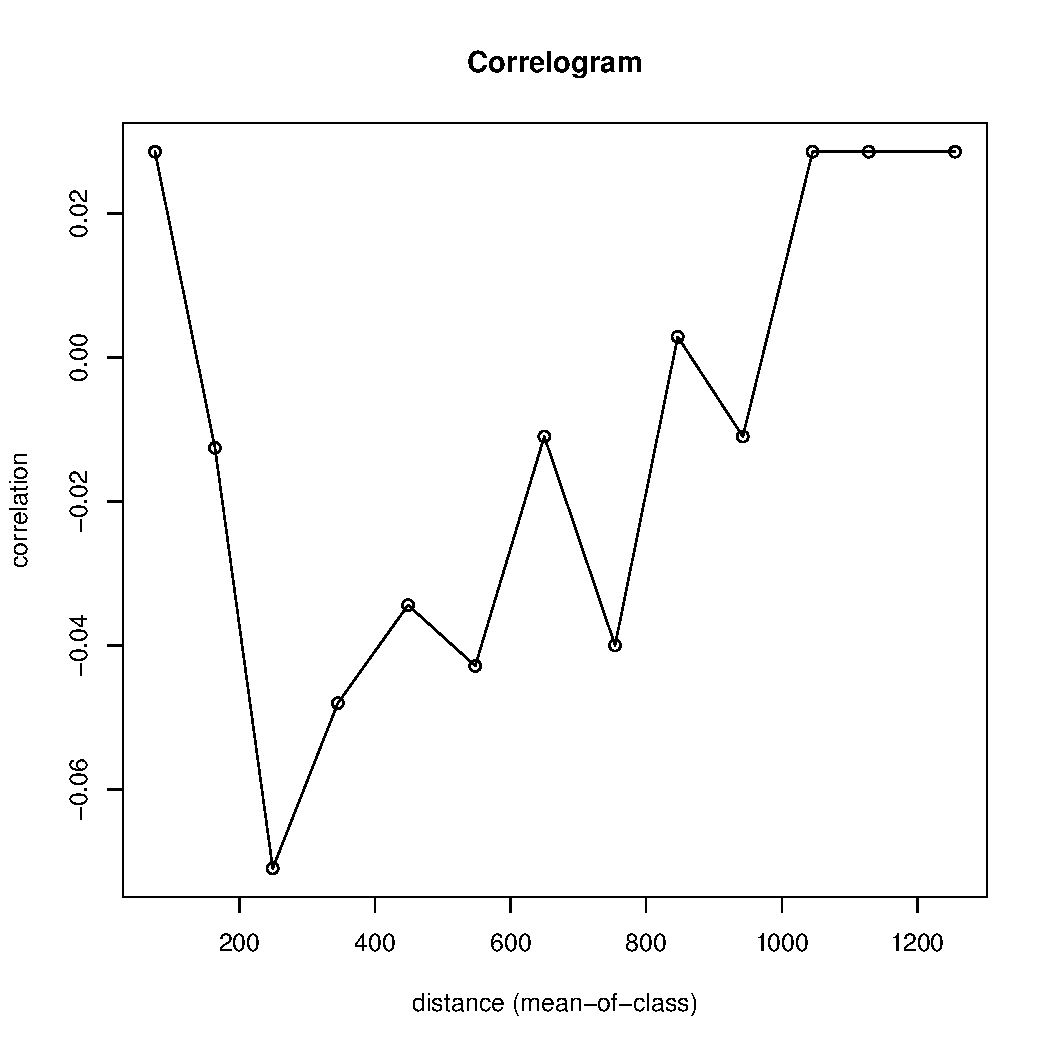
\includegraphics[width=65mm]{../Barenc_Sea/distribution_Moran/Plyazh081_moran_N_Priapulus_caudatus_.pdf}
	\end{center}
	\end{minipage}
%
	\hfil %Это пружинка отодвигающая рисунки друг от друга
%
	\begin{minipage}[b]{.46\linewidth}
%Следующий рисунок - первый ряд справа %DUNGEON S_4 \ AB
	\begin{center}
	{\small B~{\it Priapulus caudatus}}
		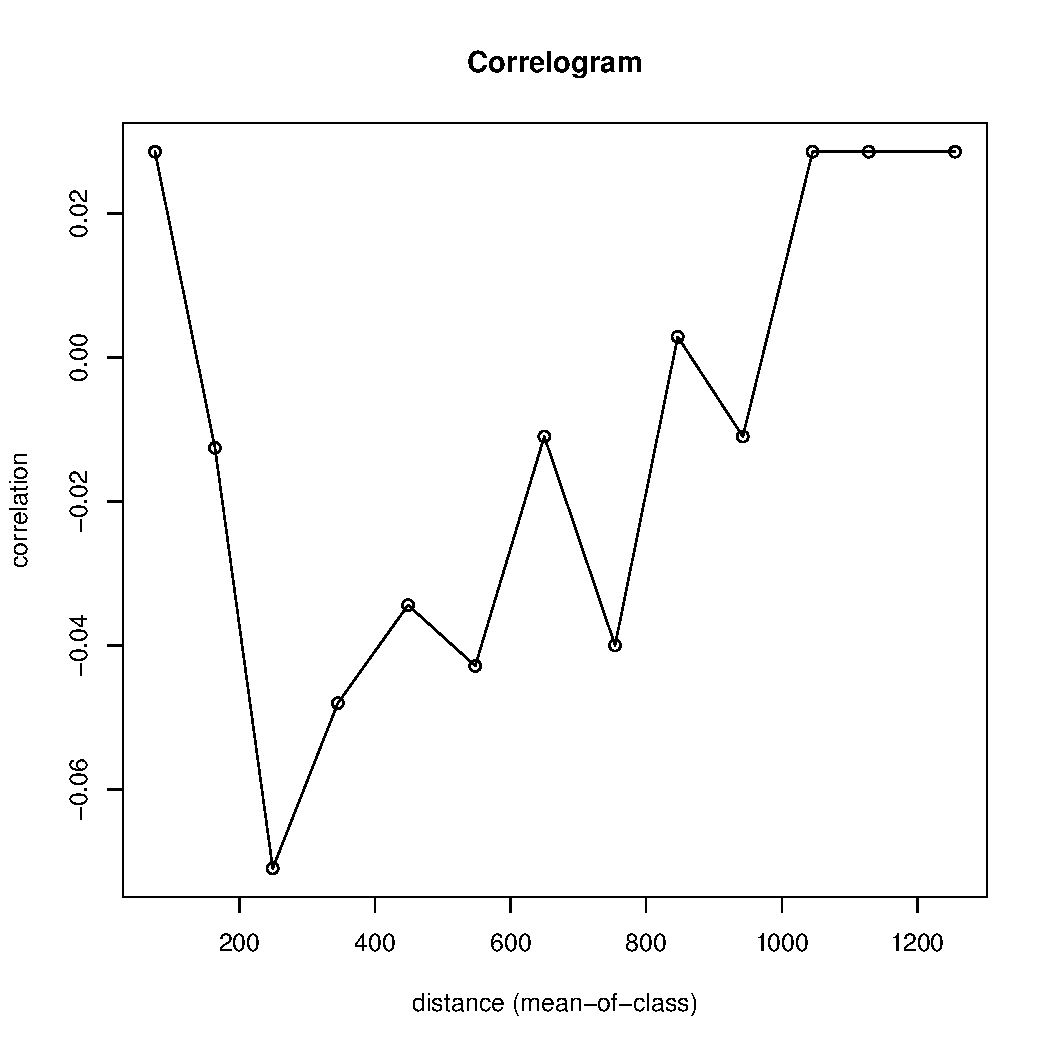
\includegraphics[width=65mm]{../Barenc_Sea/distribution_Moran/Plyazh081_moran_B_Priapulus_caudatus_.pdf}
	\end{center}
	\end{minipage}

	
%	\begin{minipage}[b]{.46\linewidth}
	%Фигурка в первом ряду слева размер отведенный под весь этот объект \textendash 0.46 от ширины строки
	%Параметр [b] означает, что выравнивание этих министраниц будет по нижнему краю
%	\begin{center}
%	{\small N~{\it Pseudolibrotus littoralis}}
%	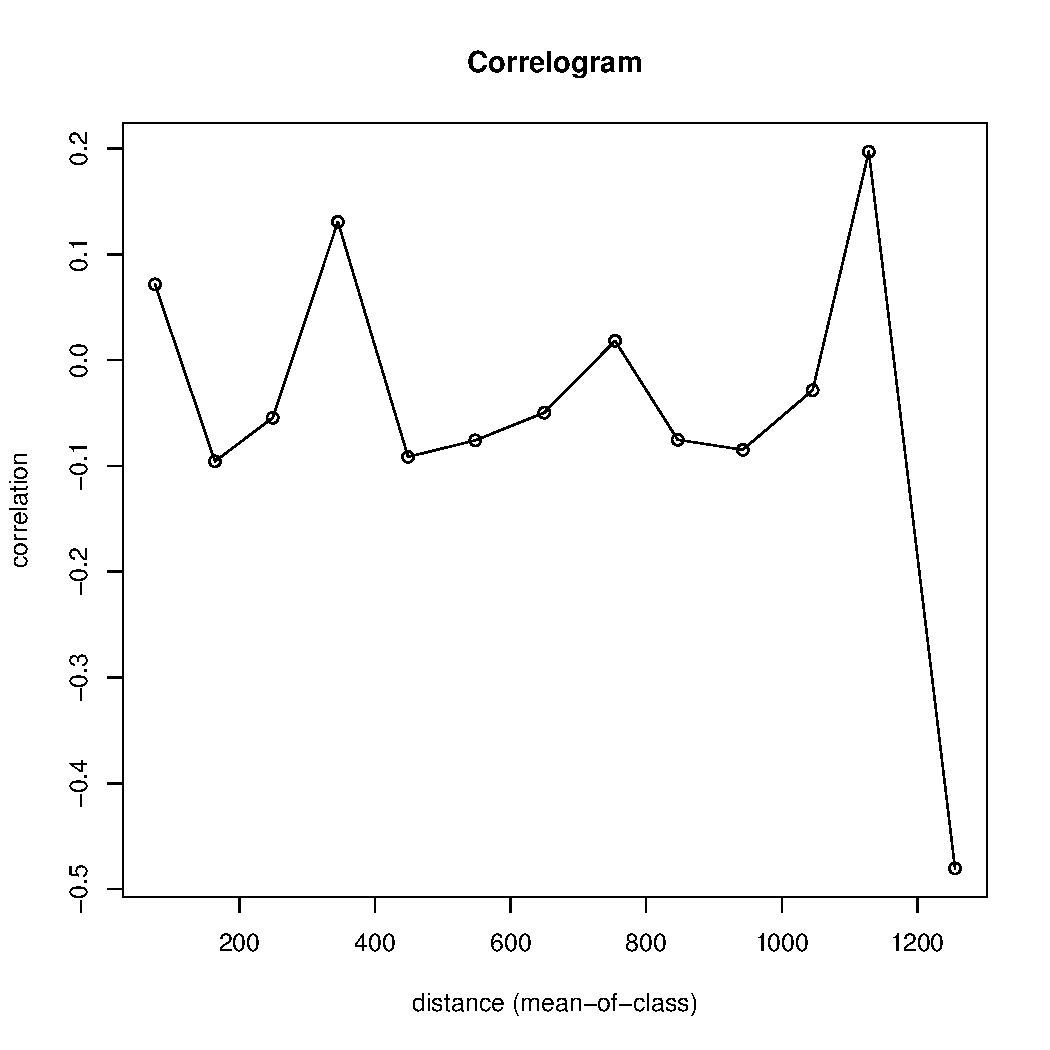
\includegraphics[width=65mm]{../Barenc_Sea/distribution_Moran/Plyazh081_moran_N_Pseudolibrotus_littoralis_.pdf}
%
%	\end{center}
%	\end{minipage}
	%
%	\hfil %Это пружинка отодвигающая рисунки друг от друга
	%
%	\begin{minipage}[b]{.46\linewidth}
%Следующий рисунок - первый ряд справа %DUNGEON S_4 \ AB
%	\begin{center}
%	{\small B~{\it Pseudolibrotus littoralis}}
%		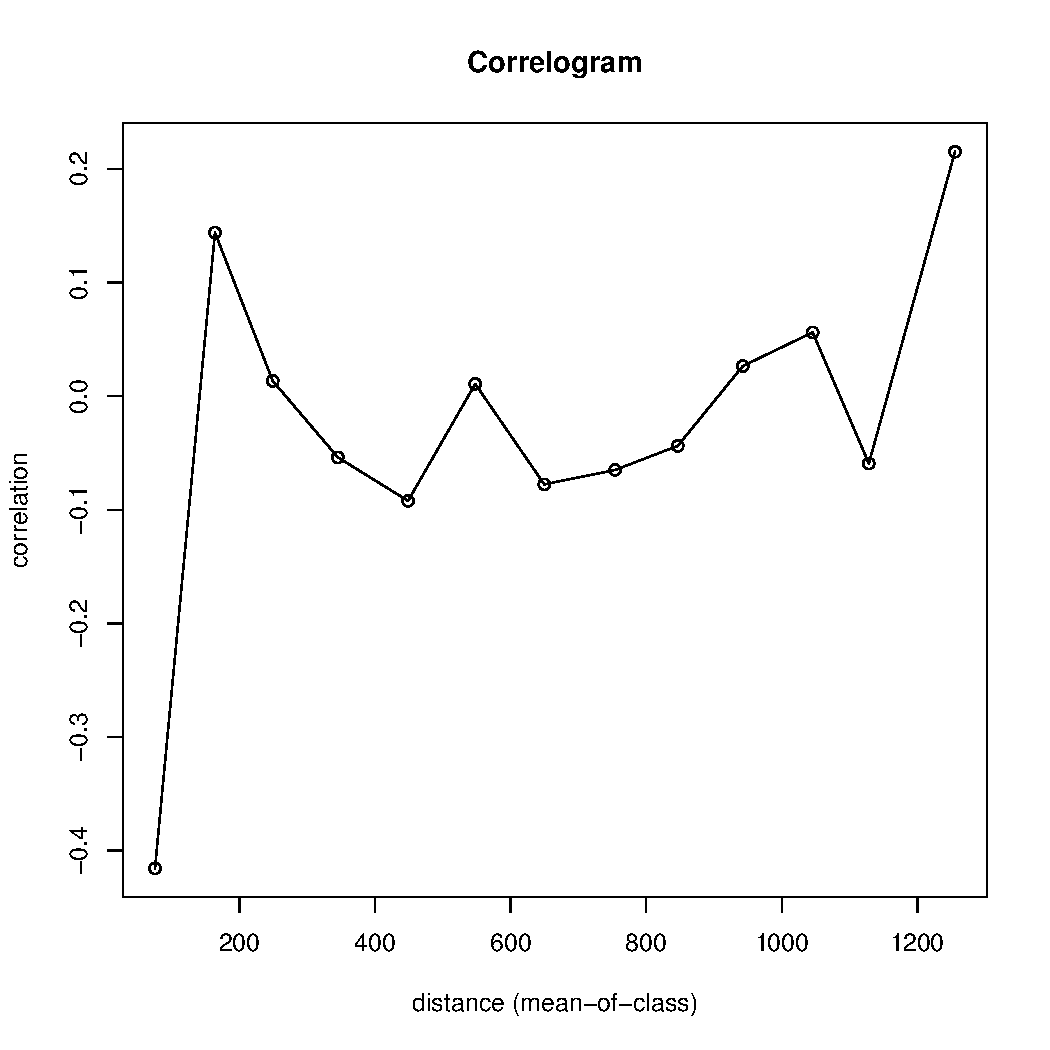
\includegraphics[width=65mm]{../Barenc_Sea/distribution_Moran/Plyazh081_moran_B_Pseudolibrotus_littoralis_.pdf}
%	\end{center}
%	\end{minipage}

%\smallskip



%\smallskip

%	\begin{minipage}[b]{.46\linewidth}
%Фигурка в первом ряду слева размер отведенный под весь этот объект \textendash 0.46 от ширины строки
%Параметр [b] означает, что выравнивание этих министраниц будет по нижнему краю
%	\begin{center}
%	{\small N~{\it Gammarus sp.}}
%		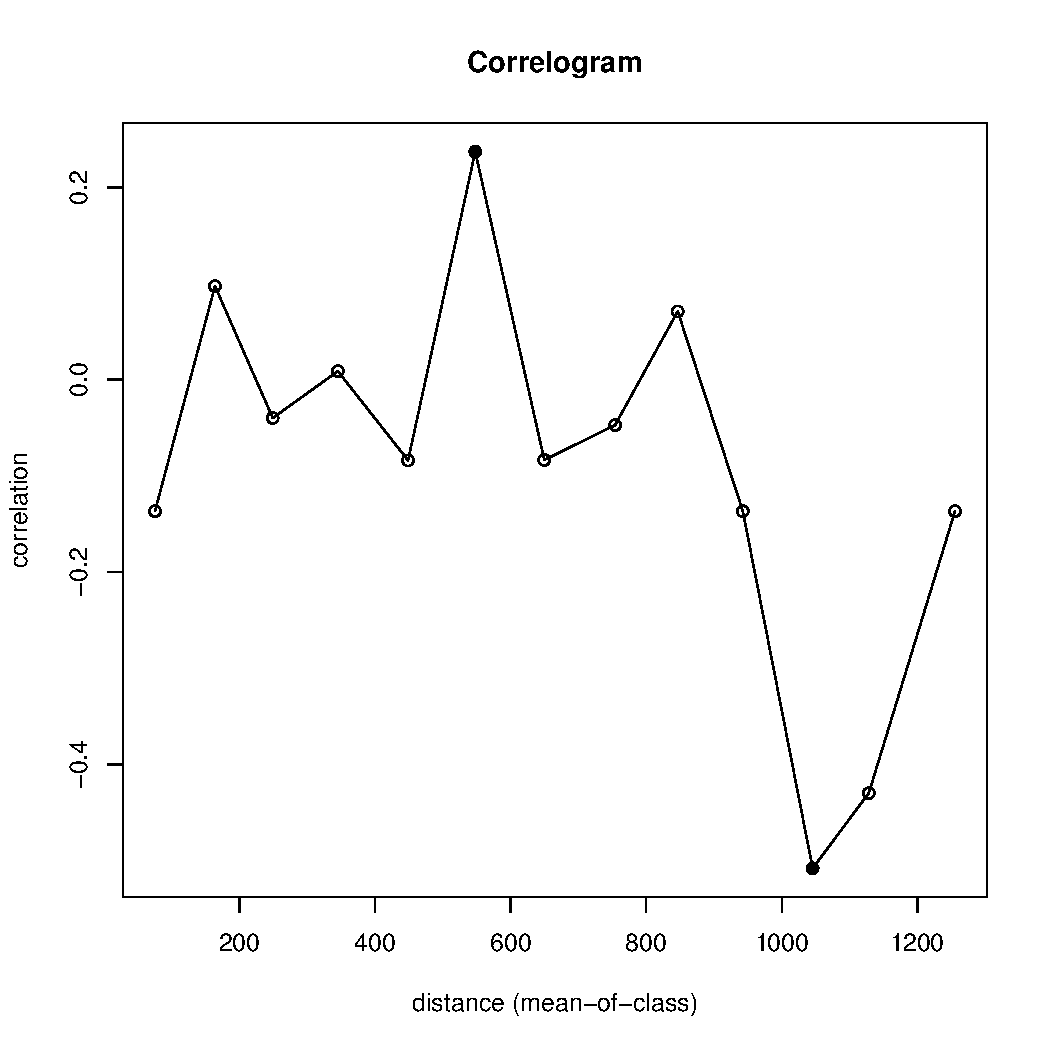
\includegraphics[width=65mm]{../Barenc_Sea/distribution_Moran/Plyazh081_moran_N_Gammarus_sp_.pdf}
%	\end{center}
%	\end{minipage}
%
%	\hfil %Это пружинка отодвигающая рисунки друг от друга
%
%	\begin{minipage}[b]{.46\linewidth}
%Следующий рисунок - первый ряд справа %DUNGEON S_4 \ AB
%	\begin{center}
%	{\small B~{\it Gammarus sp.}}
%		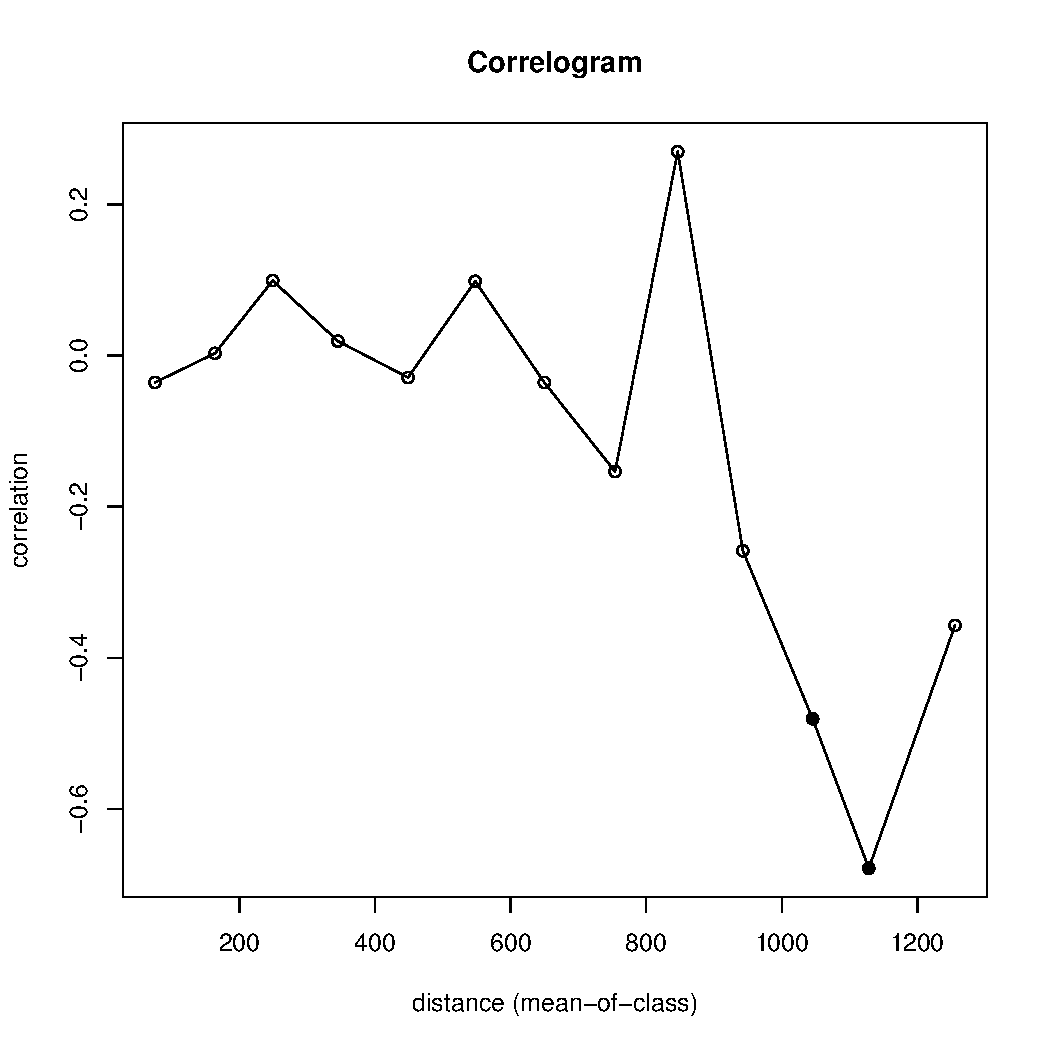
\includegraphics[width=65mm]{../Barenc_Sea/distribution_Moran/Plyazh081_moran_B_Gammarus_sp_.pdf}
%	\end{center}
%	\end{minipage}

%\smallskip


%	\caption{Микрораспределение макробентоса на литорали Дальнего пляжа г.~Дальнезеленецкая в 2007 году (продолжение).}
%	\label{ris:moransI_Plyazh081_1}
%	\end{figure}
	\begin{center}
	Рис. \ref{ris:moransI_Plyazh081_1} (продолжение). Микрораспределение макробентоса на 1 участке литорали Дальнего пляжа г.~Дальнезеленецкая в 2008 году.
	\end{center}
\end{figure}


	\begin{figure}[h]

	\begin{minipage}[b]{.46\linewidth}
%Фигурка в первом ряду слева размер отведенный под весь этот объект \textendash 0.46 от ширины строки
%Параметр [b] означает, что выравнивание этих министраниц будет по нижнему краю
	\begin{center}
	{\small N~{\it Macoma balthica}}
		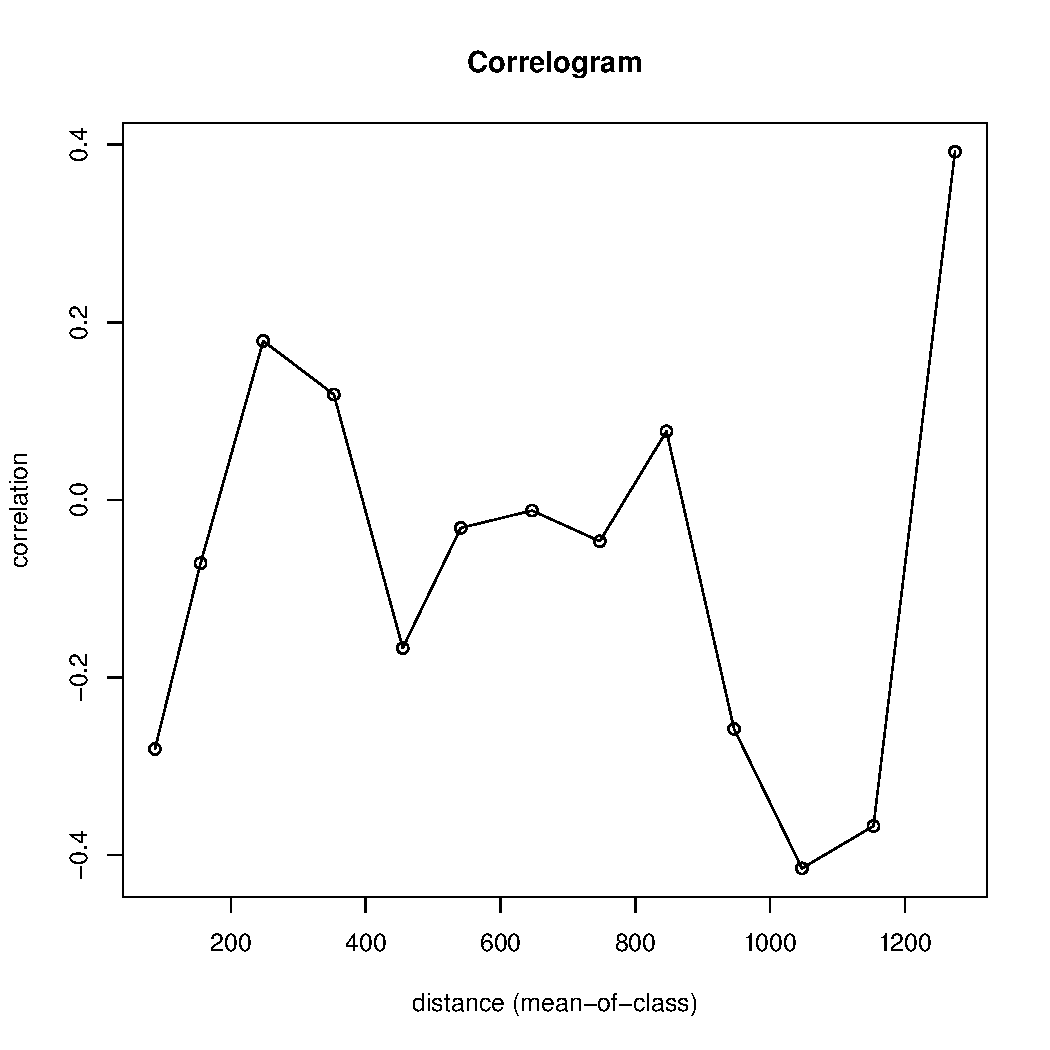
\includegraphics[width=65mm]{../Barenc_Sea/distribution_Moran/Plyazh082_moran_N_Macoma_balthica_.pdf}
	\end{center}
	\end{minipage}
%
	\hfil %Это пружинка отодвигающая рисунки друг от друга
%
	\begin{minipage}[b]{.46\linewidth}
%Следующий рисунок - первый ряд справа %DUNGEON S_4 \ AB
	\begin{center}
	{\small B~{\it Macoma balthica}}
		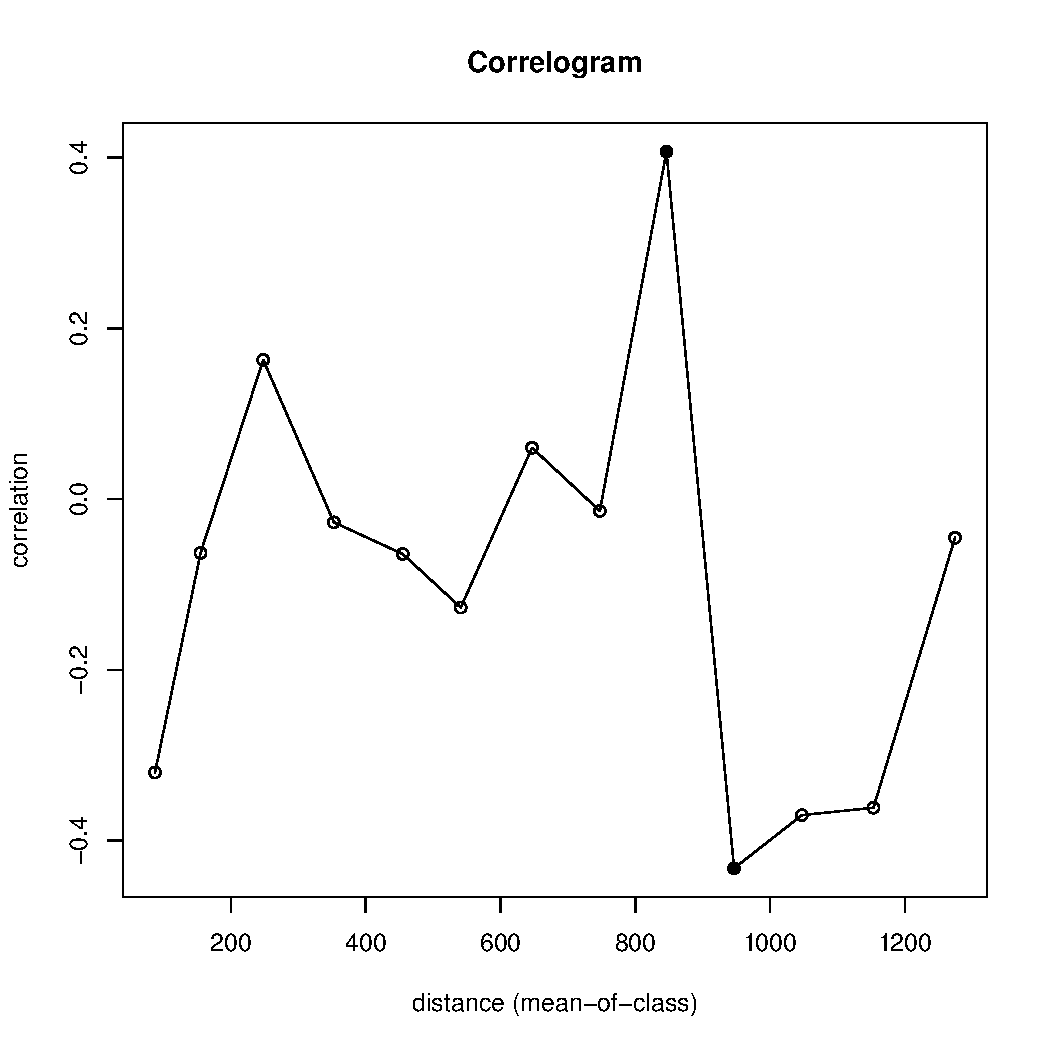
\includegraphics[width=65mm]{../Barenc_Sea/distribution_Moran/Plyazh082_moran_B_Macoma_balthica_.pdf}
	\end{center}
	\end{minipage}

	
	\begin{minipage}[b]{.46\linewidth}
	%Фигурка в первом ряду слева размер отведенный под весь этот объект \textendash 0.46 от ширины строки
	%Параметр [b] означает, что выравнивание этих министраниц будет по нижнему краю
	\begin{center}
	{\small N~{\it Cerastoderma edule}}
		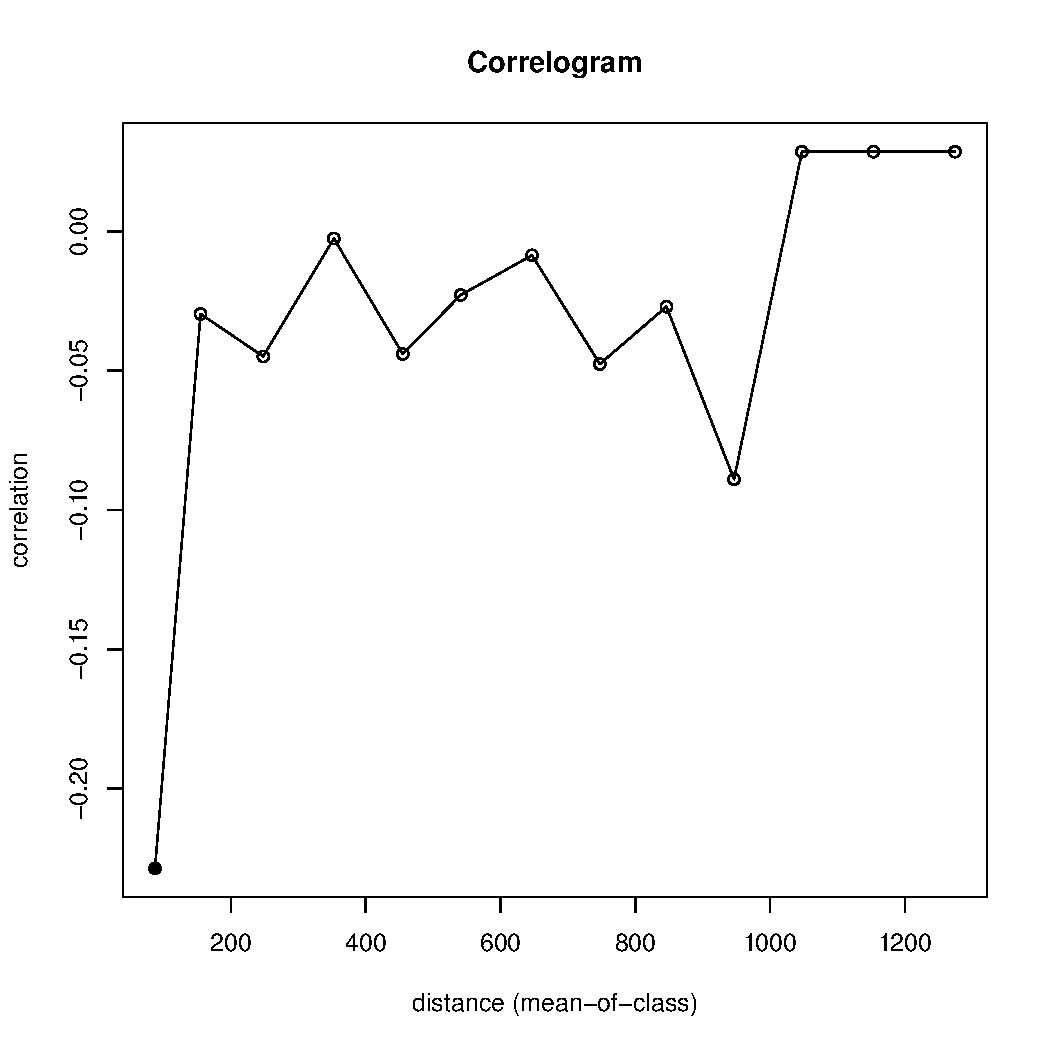
\includegraphics[width=65mm]{../Barenc_Sea/distribution_Moran/Plyazh082_moran_B_Cerastoderma_edule_.pdf}

	\end{center}
	\end{minipage}
	%
	\hfil %Это пружинка отодвигающая рисунки друг от друга
	%
	\begin{minipage}[b]{.46\linewidth}
%Следующий рисунок - первый ряд справа %DUNGEON S_4 \ AB
	\begin{center}
	{\small B~{\it Cerastoderma edule}}
		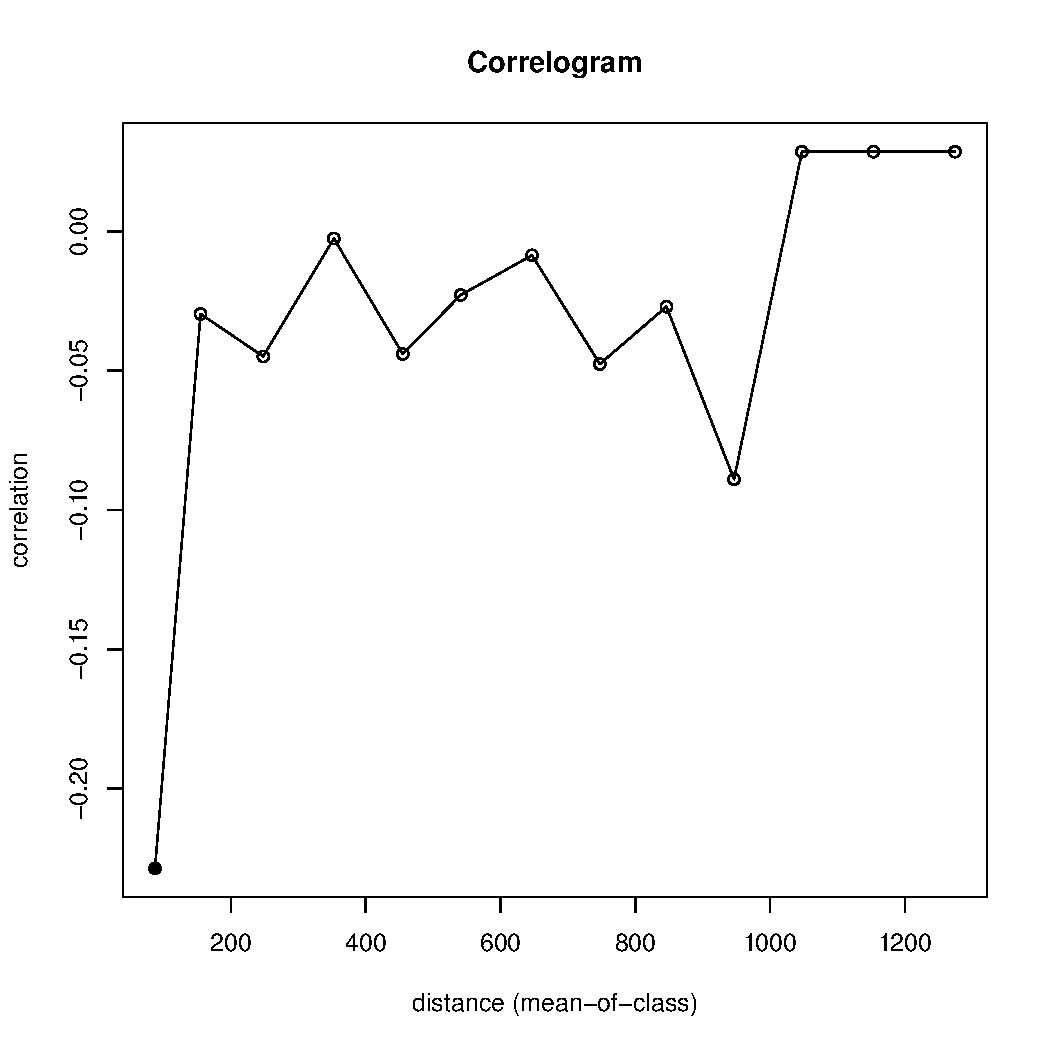
\includegraphics[width=65mm]{../Barenc_Sea/distribution_Moran/Plyazh082_moran_B_Cerastoderma_edule_.pdf}
	\end{center}
	\end{minipage}

%\smallskip



%\smallskip

	\begin{minipage}[b]{.46\linewidth}
%Фигурка в первом ряду слева размер отведенный под весь этот объект \textendash 0.46 от ширины строки
%Параметр [b] означает, что выравнивание этих министраниц будет по нижнему краю
	\begin{center}
	{\small N~{\it Mya arenaria}}
		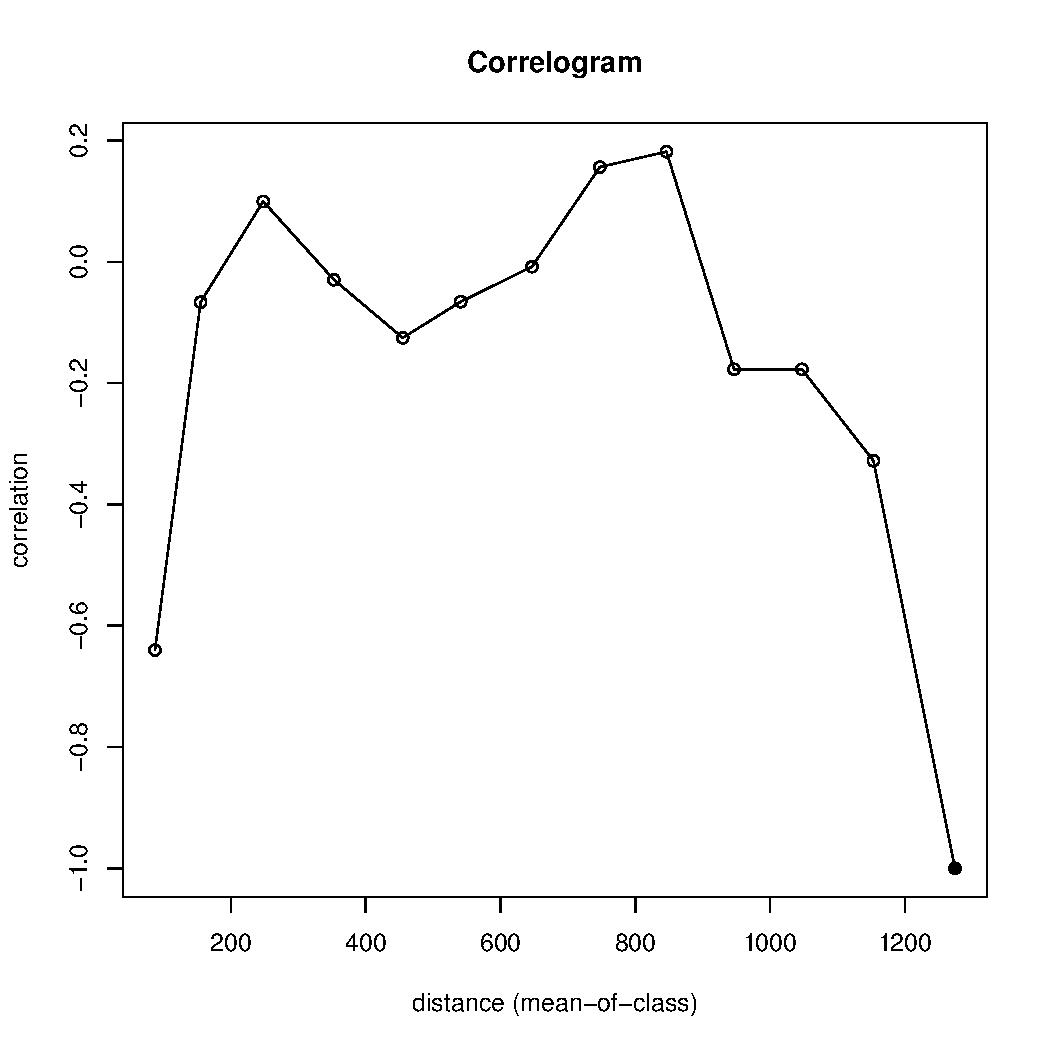
\includegraphics[width=65mm]{../Barenc_Sea/distribution_Moran/Plyazh082_moran_N_Mya_arenaria_.pdf}
	\end{center}
	\end{minipage}
%
	\hfil %Это пружинка отодвигающая рисунки друг от друга
%
	\begin{minipage}[b]{.46\linewidth}
%Следующий рисунок - первый ряд справа %DUNGEON S_4 \ AB
	\begin{center}
	{\small B~{\it Mya arenaria}}
		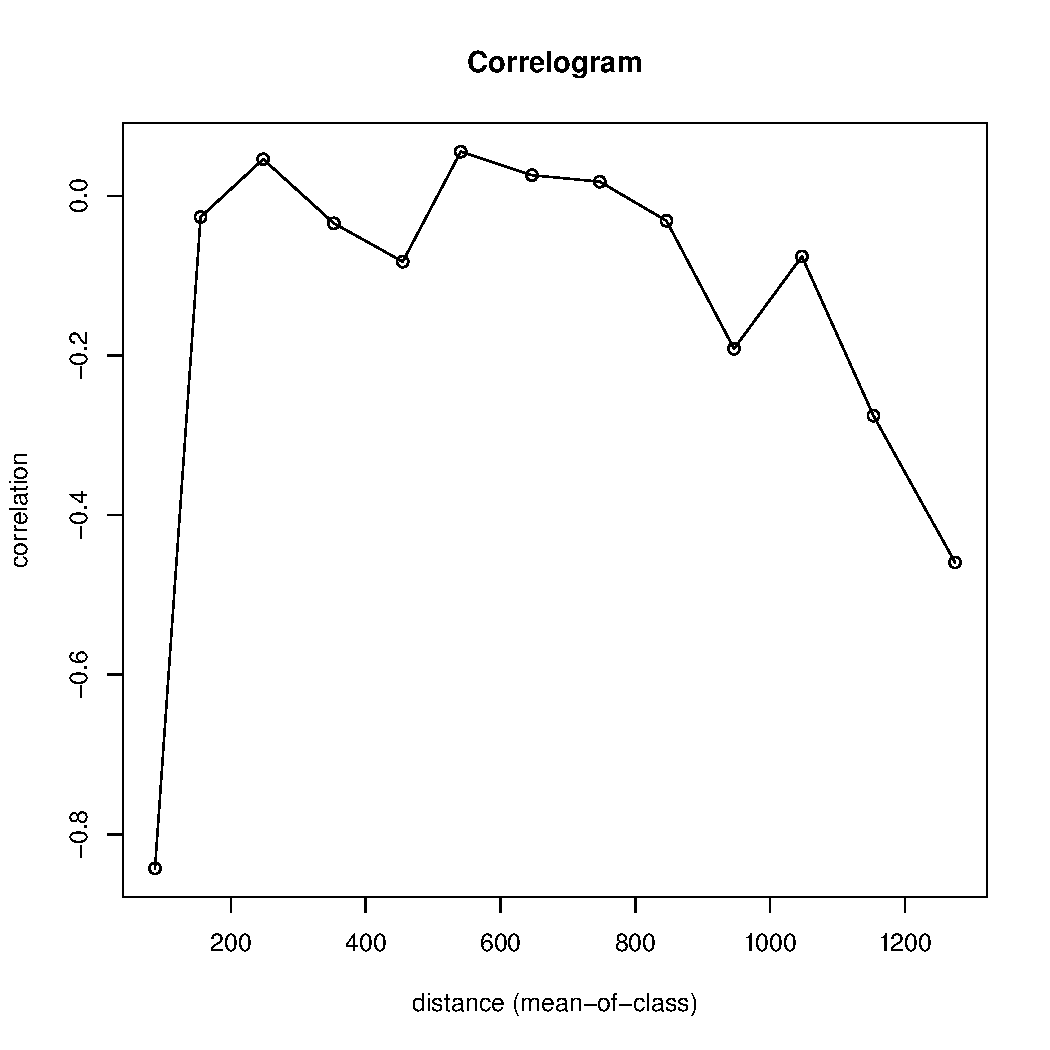
\includegraphics[width=65mm]{../Barenc_Sea/distribution_Moran/Plyazh082_moran_B_Mya_arenaria_.pdf}
	\end{center}
	\end{minipage}

%\smallskip


	\caption{Микрораспределение макробентоса на 2 участке на литорали Дальнего пляжа г.~Дальнезеленецкая в 2008 году.}
	\label{ris:moransI_Plyazh082_1}
	\end{figure}



	\begin{figure}[h]

	\begin{minipage}[b]{.46\linewidth}
%Фигурка в первом ряду слева размер отведенный под весь этот объект \textendash 0.46 от ширины строки
%Параметр [b] означает, что выравнивание этих министраниц будет по нижнему краю
	\begin{center}
	{\small N~{\it Mytilus edulis}}
		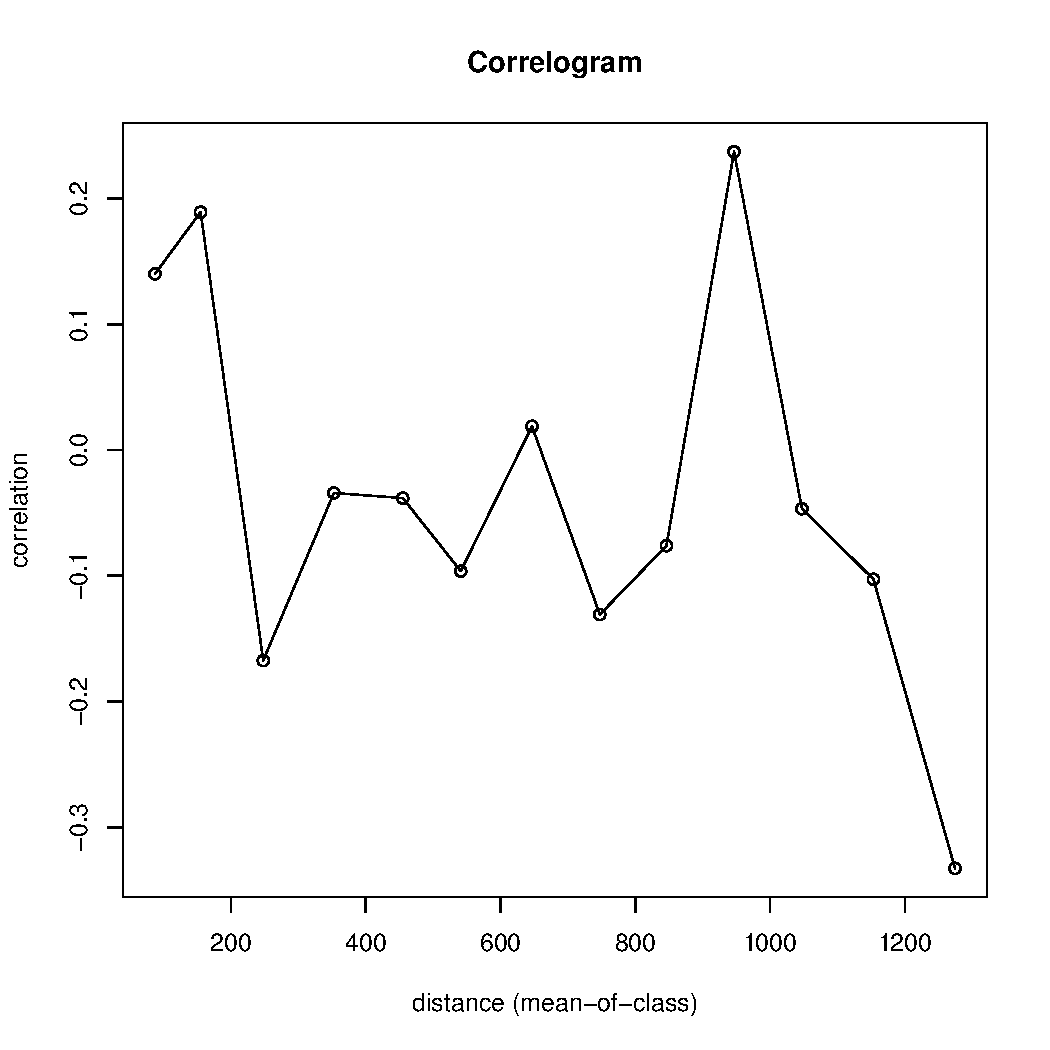
\includegraphics[width=65mm]{../Barenc_Sea/distribution_Moran/Plyazh082_moran_N_Mytilus_edulis_.pdf}
	\end{center}
	\end{minipage}
%
	\hfil %Это пружинка отодвигающая рисунки друг от друга
%
	\begin{minipage}[b]{.46\linewidth}
%Следующий рисунок - первый ряд справа %DUNGEON S_4 \ AB
	\begin{center}
	{\small B~{\it Mytilus edulis}}
		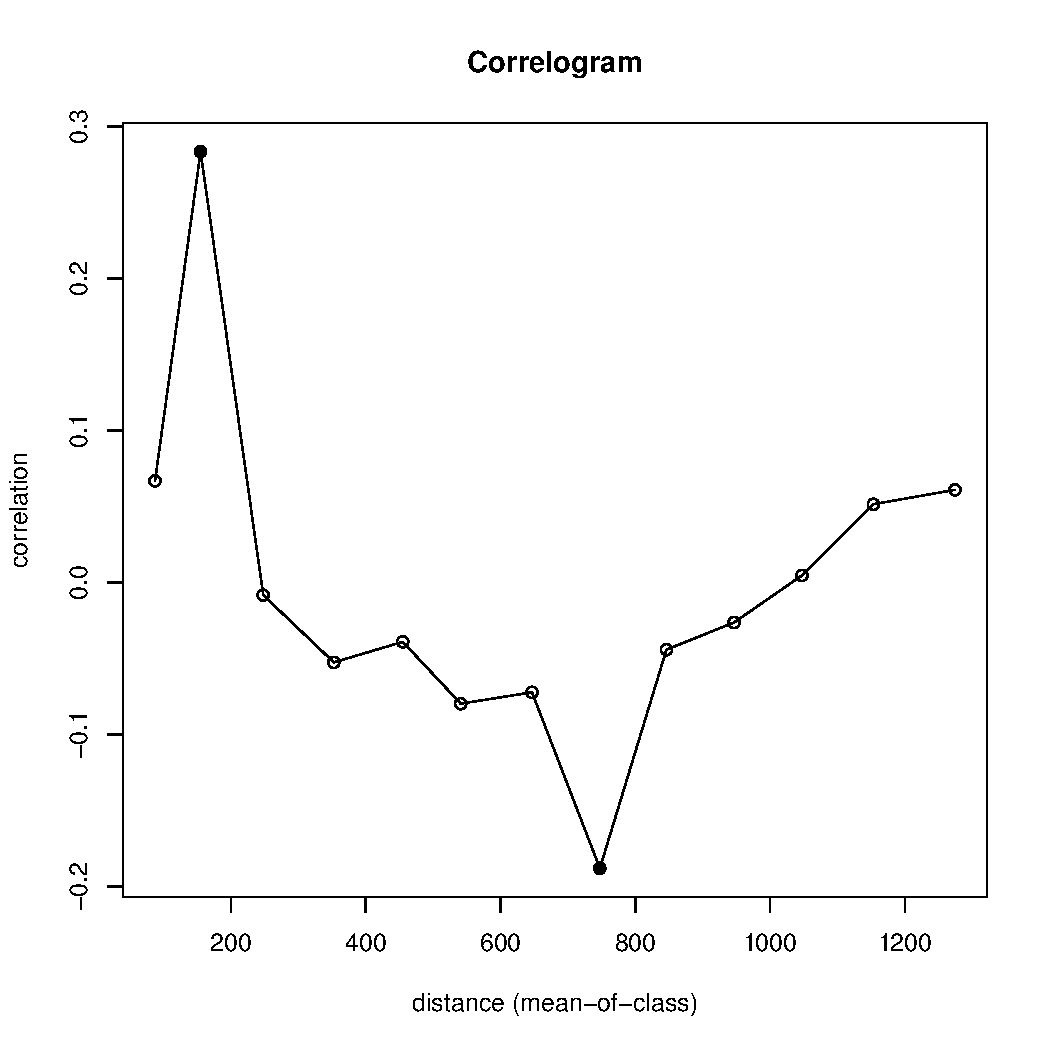
\includegraphics[width=65mm]{../Barenc_Sea/distribution_Moran/Plyazh082_moran_B_Mytilus_edulis_.pdf}
	\end{center}
	\end{minipage}

	
	\begin{minipage}[b]{.46\linewidth}
	%Фигурка в первом ряду слева размер отведенный под весь этот объект \textendash 0.46 от ширины строки
	%Параметр [b] означает, что выравнивание этих министраниц будет по нижнему краю
	\begin{center}
	{\small N~{\it Pseudolibrotus littoralis}}
	\includegraphics[width=65mm]{../Barenc_Sea/distribution_Moran/Plyazh082_moran_N_Pseudolibrotus_littoralis_.pdf}

	\end{center}
	\end{minipage}
	%
	\hfil %Это пружинка отодвигающая рисунки друг от друга
	%
	\begin{minipage}[b]{.46\linewidth}
%Следующий рисунок - первый ряд справа %DUNGEON S_4 \ AB
	\begin{center}
	{\small B~{\it Pseudolibrotus littoralis}}
		\includegraphics[width=65mm]{../Barenc_Sea/distribution_Moran/Plyazh082_moran_B_Pseudolibrotus_littoralis_.pdf}
	\end{center}
	\end{minipage}

%\smallskip



%\smallskip

%	\begin{minipage}[b]{.46\linewidth}
%Фигурка в первом ряду слева размер отведенный под весь этот объект \textendash 0.46 от ширины строки
%Параметр [b] означает, что выравнивание этих министраниц будет по нижнему краю
%	\begin{center}
%	{\small N~{\it Gammarus sp.}}
%		\includegraphics[width=65mm]{../Barenc_Sea/distribution_Moran/Plyazh082_moran_N_Gammarus_sp_.pdf}
%	\end{center}
%	\end{minipage}
%
%	\hfil %Это пружинка отодвигающая рисунки друг от друга
%
%	\begin{minipage}[b]{.46\linewidth}
%Следующий рисунок - первый ряд справа %DUNGEON S_4 \ AB
%	\begin{center}
%	{\small B~{\it Gammarus sp.}}
%		\includegraphics[width=65mm]{../Barenc_Sea/distribution_Moran/Plyazh082_moran_B_Gammarus_sp_.pdf}
%	\end{center}
%	\end{minipage}

%\smallskip


%	\caption{Микрораспределение макробентоса на литорали Дальнего пляжа г.~Дальнезеленецкая в 2007 году (продолжение).}
%	\label{ris:moransI_Plyazh082_1}
%	\end{figure}
	\begin{center}
	Рис. \ref{ris:moransI_Plyazh082_1} (продолжение). Микрораспределение макробентоса на 2 участке литорали Дальнего пляжа г.~Дальнезеленецкая в 2008 году.
	\end{center}

\end{figure}



	\begin{figure}[h]

	\begin{minipage}[b]{.46\linewidth}
%Фигурка в первом ряду слева размер отведенный под весь этот объект \textendash 0.46 от ширины строки
%Параметр [b] означает, что выравнивание этих министраниц будет по нижнему краю
	\begin{center}
	{\small N~{\it Macoma balthica}}
		\includegraphics[width=65mm]{../Barenc_Sea/distribution_Moran/Plyazh0812_moran_N_Macoma_balthica_.pdf}
	\end{center}
	\end{minipage}
%
	\hfil %Это пружинка отодвигающая рисунки друг от друга
%
	\begin{minipage}[b]{.46\linewidth}
%Следующий рисунок - первый ряд справа %DUNGEON S_4 \ AB
	\begin{center}
	{\small B~{\it Macoma balthica}}
		\includegraphics[width=65mm]{../Barenc_Sea/distribution_Moran/Plyazh0812_moran_B_Macoma_balthica_.pdf}
	\end{center}
	\end{minipage}

	
	\begin{minipage}[b]{.46\linewidth}
	%Фигурка в первом ряду слева размер отведенный под весь этот объект \textendash 0.46 от ширины строки
	%Параметр [b] означает, что выравнивание этих министраниц будет по нижнему краю
	\begin{center}
	{\small N~{\it Cerastoderma edule}}
		\includegraphics[width=65mm]{../Barenc_Sea/distribution_Moran/Plyazh0812_moran_B_Cerastoderma_edule_.pdf}

	\end{center}
	\end{minipage}
	%
	\hfil %Это пружинка отодвигающая рисунки друг от друга
	%
	\begin{minipage}[b]{.46\linewidth}
%Следующий рисунок - первый ряд справа %DUNGEON S_4 \ AB
	\begin{center}
	{\small B~{\it Cerastoderma edule}}
		\includegraphics[width=65mm]{../Barenc_Sea/distribution_Moran/Plyazh0812_moran_B_Cerastoderma_edule_.pdf}
	\end{center}
	\end{minipage}

%\smallskip



%\smallskip

	\begin{minipage}[b]{.46\linewidth}
%Фигурка в первом ряду слева размер отведенный под весь этот объект \textendash 0.46 от ширины строки
%Параметр [b] означает, что выравнивание этих министраниц будет по нижнему краю
	\begin{center}
	{\small N~{\it Mya arenaria}}
		\includegraphics[width=65mm]{../Barenc_Sea/distribution_Moran/Plyazh0812_moran_N_Mya_arenaria_.pdf}
	\end{center}
	\end{minipage}
%
	\hfil %Это пружинка отодвигающая рисунки друг от друга
%
	\begin{minipage}[b]{.46\linewidth}
%Следующий рисунок - первый ряд справа %DUNGEON S_4 \ AB
	\begin{center}
	{\small B~{\it Mya arenaria}}
		\includegraphics[width=65mm]{../Barenc_Sea/distribution_Moran/Plyazh0812_moran_B_Mya_arenaria_.pdf}
	\end{center}
	\end{minipage}

%\smallskip


	\caption{Микрораспределение макробентоса на объединенном участке на литорали Дальнего пляжа г.~Дальнезеленецкая в 2008 году.}
	\label{ris:moransI_Plyazh0812_1}
	\end{figure}



	\begin{figure}[h]

	\begin{minipage}[b]{.46\linewidth}
%Фигурка в первом ряду слева размер отведенный под весь этот объект \textendash 0.46 от ширины строки
%Параметр [b] означает, что выравнивание этих министраниц будет по нижнему краю
	\begin{center}
	{\small N~{\it Mytilus edulis}}
		\includegraphics[width=65mm]{../Barenc_Sea/distribution_Moran/Plyazh0812_moran_N_Mytilus_edulis_.pdf}
	\end{center}
	\end{minipage}
%
	\hfil %Это пружинка отодвигающая рисунки друг от друга
%
	\begin{minipage}[b]{.46\linewidth}
%Следующий рисунок - первый ряд справа %DUNGEON S_4 \ AB
	\begin{center}
	{\small B~{\it Mytilus edulis}}
		\includegraphics[width=65mm]{../Barenc_Sea/distribution_Moran/Plyazh0812_moran_B_Mytilus_edulis_.pdf}
	\end{center}
	\end{minipage}

	
	\begin{minipage}[b]{.46\linewidth}
	%Фигурка в первом ряду слева размер отведенный под весь этот объект \textendash 0.46 от ширины строки
	%Параметр [b] означает, что выравнивание этих министраниц будет по нижнему краю
	\begin{center}
	{\small N~{\it Pseudolibrotus littoralis}}
	\includegraphics[width=65mm]{../Barenc_Sea/distribution_Moran/Plyazh0812_moran_N_Pseudolibrotus_littoralis_.pdf}

	\end{center}
	\end{minipage}
	%
	\hfil %Это пружинка отодвигающая рисунки друг от друга
	%
	\begin{minipage}[b]{.46\linewidth}
%Следующий рисунок - первый ряд справа %DUNGEON S_4 \ AB
	\begin{center}
	{\small B~{\it Pseudolibrotus littoralis}}
		\includegraphics[width=65mm]{../Barenc_Sea/distribution_Moran/Plyazh0812_moran_B_Pseudolibrotus_littoralis_.pdf}
	\end{center}
	\end{minipage}

%\smallskip



%\smallskip

	\begin{minipage}[b]{.46\linewidth}
%Фигурка в первом ряду слева размер отведенный под весь этот объект \textendash 0.46 от ширины строки
%Параметр [b] означает, что выравнивание этих министраниц будет по нижнему краю
	\begin{center}
	{\small N~{\it Gammarus sp.}}
		\includegraphics[width=65mm]{../Barenc_Sea/distribution_Moran/Plyazh0812_moran_N_Gammarus_sp_.pdf}
	\end{center}
	\end{minipage}
%
	\hfil %Это пружинка отодвигающая рисунки друг от друга
%
%	\begin{minipage}[b]{.46\linewidth}
%Следующий рисунок - первый ряд справа %DUNGEON S_4 \ AB
	\begin{center}
	{\small B~{\it Gammarus sp.}}
		\includegraphics[width=65mm]{../Barenc_Sea/distribution_Moran/Plyazh0812_moran_B_Gammarus_sp_.pdf}
	\end{center}
	\end{minipage}

%\smallskip


%	\caption{Микрораспределение макробентоса на литорали Дальнего пляжа г.~Дальнезеленецкая в 2007 году (продолжение).}
%	\label{ris:moransI_Plyazh0812_1}
%	\end{figure}
	\begin{center}
	Рис. \ref{ris:moransI_Plyazh081_1} (продолжение). Микрораспределение макробентоса на объединенном участке литорали Дальнего пляжа г.~Дальнезеленецкая в 2008 году.
	\end{center}

\end{figure}


	\begin{figure}[h]

	\begin{minipage}[b]{.46\linewidth}
%Фигурка в первом ряду слева размер отведенный под весь этот объект \textendash 0.46 от ширины строки
%Параметр [b] означает, что выравнивание этих министраниц будет по нижнему краю
	\begin{center}
	{\small N~{\it Priapulus caudatus}}
		\includegraphics[width=65mm]{../Barenc_Sea/distribution_Moran/Plyazh0812_moran_N_Priapulus_caudatus_.pdf}
	\end{center}
	\end{minipage}
%
	\hfil %Это пружинка отодвигающая рисунки друг от друга
%
	\begin{minipage}[b]{.46\linewidth}
%Следующий рисунок - первый ряд справа %DUNGEON S_4 \ AB
	\begin{center}
	{\small B~{\it Priapulus caudatus}}
		\includegraphics[width=65mm]{../Barenc_Sea/distribution_Moran/Plyazh0812_moran_B_Priapulus_caudatus_.pdf}
	\end{center}
	\end{minipage}

	
%	\begin{minipage}[b]{.46\linewidth}
	%Фигурка в первом ряду слева размер отведенный под весь этот объект \textendash 0.46 от ширины строки
	%Параметр [b] означает, что выравнивание этих министраниц будет по нижнему краю
%	\begin{center}
%	{\small N~{\it Pseudolibrotus littoralis}}
%	\includegraphics[width=65mm]{../Barenc_Sea/distribution_Moran/Plyazh0812_moran_N_Pseudolibrotus_littoralis_.pdf}
%
%	\end{center}
%	\end{minipage}
	%
%	\hfil %Это пружинка отодвигающая рисунки друг от друга
	%
%	\begin{minipage}[b]{.46\linewidth}
%Следующий рисунок - первый ряд справа %DUNGEON S_4 \ AB
%	\begin{center}
%	{\small B~{\it Pseudolibrotus littoralis}}
%		\includegraphics[width=65mm]{../Barenc_Sea/distribution_Moran/Plyazh0812_moran_B_Pseudolibrotus_littoralis_.pdf}
%	\end{center}
%	\end{minipage}

%\smallskip



%\smallskip

%	\begin{minipage}[b]{.46\linewidth}
%Фигурка в первом ряду слева размер отведенный под весь этот объект \textendash 0.46 от ширины строки
%Параметр [b] означает, что выравнивание этих министраниц будет по нижнему краю
%	\begin{center}
%	{\small N~{\it Gammarus sp.}}
%		\includegraphics[width=65mm]{../Barenc_Sea/distribution_Moran/Plyazh0812_moran_N_Gammarus_sp_.pdf}
%	\end{center}
%	\end{minipage}
%
%	\hfil %Это пружинка отодвигающая рисунки друг от друга
%
%	\begin{minipage}[b]{.46\linewidth}
%Следующий рисунок - первый ряд справа %DUNGEON S_4 \ AB
%	\begin{center}
%	{\small B~{\it Gammarus sp.}}
%		\includegraphics[width=65mm]{../Barenc_Sea/distribution_Moran/Plyazh0812_moran_B_Gammarus_sp_.pdf}
%	\end{center}
%	\end{minipage}

%\smallskip


%	\caption{Микрораспределение макробентоса на литорали Дальнего пляжа г.~Дальнезеленецкая в 2007 году (продолжение).}
%	\label{ris:moransI_Plyazh0812_1}
%	\end{figure}
	\begin{center}
	Рис. \ref{ris:moransI_Plyazh0812_1} (продолжение). Микрораспределение макробентоса на объединенном участке литорали Дальнего пляжа г.~Дальнезеленецкая в 2008 году.
	\end{center}
  \end{figure}


	\begin{figure}[h]

	\begin{minipage}[b]{.46\linewidth}
%Фигурка в первом ряду слева размер отведенный под весь этот объект \textendash 0.46 от ширины строки
%Параметр [b] означает, что выравнивание этих министраниц будет по нижнему краю
	\begin{center}
	{\small N~{\it Macoma balthica}}
		\includegraphics[width=65mm]{../Barenc_Sea/distribution_Moran/Yarnyshnaya07_moran_N_Macoma_balthica_.pdf}
	\end{center}
	\end{minipage}
%
	\hfil %Это пружинка отодвигающая рисунки друг от друга
%
	\begin{minipage}[b]{.46\linewidth}
%Следующий рисунок - первый ряд справа %DUNGEON S_4 \ AB
	\begin{center}
	{\small B~{\it Macoma balthica}}
		\includegraphics[width=65mm]{../Barenc_Sea/distribution_Moran/Yarnyshnaya07_moran_B_Macoma_balthica_.pdf}
	\end{center}
	\end{minipage}

	
	\begin{minipage}[b]{.46\linewidth}
	%Фигурка в первом ряду слева размер отведенный под весь этот объект \textendash 0.46 от ширины строки
	%Параметр [b] означает, что выравнивание этих министраниц будет по нижнему краю
	\begin{center}
	{\small N~{\it Cerastoderma edule}}
		\includegraphics[width=65mm]{../Barenc_Sea/distribution_Moran/Yarnyshnaya07_moran_B_Cerastoderma_edule_.pdf}

	\end{center}
	\end{minipage}
	%
	\hfil %Это пружинка отодвигающая рисунки друг от друга
	%
	\begin{minipage}[b]{.46\linewidth}
%Следующий рисунок - первый ряд справа %DUNGEON S_4 \ AB
	\begin{center}
	{\small B~{\it Cerastoderma edule}}
		\includegraphics[width=65mm]{../Barenc_Sea/distribution_Moran/Yarnyshnaya07_moran_B_Cerastoderma_edule_.pdf}
	\end{center}
	\end{minipage}

%\smallskip



%\smallskip

	\begin{minipage}[b]{.46\linewidth}
%Фигурка в первом ряду слева размер отведенный под весь этот объект \textendash 0.46 от ширины строки
%Параметр [b] означает, что выравнивание этих министраниц будет по нижнему краю
	\begin{center}
	{\small N~{\it Mya arenaria}}
		\includegraphics[width=65mm]{../Barenc_Sea/distribution_Moran/Yarnyshnaya07_moran_N_Mya_arenaria_.pdf}
	\end{center}
	\end{minipage}
%
	\hfil %Это пружинка отодвигающая рисунки друг от друга
%
	\begin{minipage}[b]{.46\linewidth}
%Следующий рисунок - первый ряд справа %DUNGEON S_4 \ AB
	\begin{center}
	{\small B~{\it Mya arenaria}}
		\includegraphics[width=65mm]{../Barenc_Sea/distribution_Moran/Yarnyshnaya07_moran_B_Mya_arenaria_.pdf}
	\end{center}
	\end{minipage}

%\smallskip


	\caption{Микрораспределение макробентоса на литорали  г.~Ярнышная в 2007 году.}
	\label{ris:moransI_Yarn07_1}
	\end{figure}



	\begin{figure}[h]

	\begin{minipage}[b]{.46\linewidth}
%Фигурка в первом ряду слева размер отведенный под весь этот объект \textendash 0.46 от ширины строки
%Параметр [b] означает, что выравнивание этих министраниц будет по нижнему краю
	\begin{center}
	{\small N~{\it Mytilus edulis}}
		\includegraphics[width=65mm]{../Barenc_Sea/distribution_Moran/Yarnyshnaya07_moran_N_Mytilus_edulis_.pdf}
	\end{center}
	\end{minipage}
%
	\hfil %Это пружинка отодвигающая рисунки друг от друга
%
	\begin{minipage}[b]{.46\linewidth}
%Следующий рисунок - первый ряд справа %DUNGEON S_4 \ AB
	\begin{center}
	{\small B~{\it Mytilus edulis}}
		\includegraphics[width=65mm]{../Barenc_Sea/distribution_Moran/Yarnyshnaya07_moran_B_Mytilus_edulis_.pdf}
	\end{center}
	\end{minipage}

	
%	\begin{minipage}[b]{.46\linewidth}
	%Фигурка в первом ряду слева размер отведенный под весь этот объект \textendash 0.46 от ширины строки
	%Параметр [b] означает, что выравнивание этих министраниц будет по нижнему краю
%	\begin{center}
%	{\small N~{\it Pseudolibrotus littoralis}}
%	\includegraphics[width=65mm]{../Barenc_Sea/distribution_Moran/Yarnyshnaya07_moran_N_Pseudolibrotus_littoralis_.pdf}

%	\end{center}
%	\end{minipage}
	%
%	\hfil %Это пружинка отодвигающая рисунки друг от друга
%	%
%	\begin{minipage}[b]{.46\linewidth}
%Следующий рисунок - первый ряд справа %DUNGEON S_4 \ AB
%	\begin{center}
%	{\small B~{\it Pseudolibrotus littoralis}}
%		\includegraphics[width=65mm]{../Barenc_Sea/distribution_Moran/Yarnyshnaya07_moran_B_Pseudolibrotus_littoralis_.pdf}
%	\end{center}
%	\end{minipage}

%\smallskip



%\smallskip

%	\begin{minipage}[b]{.46\linewidth}
%Фигурка в первом ряду слева размер отведенный под весь этот объект \textendash 0.46 от ширины строки
%Параметр [b] означает, что выравнивание этих министраниц будет по нижнему краю
%	\begin{center}
%	{\small N~{\it Gammarus sp.}}
%		\includegraphics[width=65mm]{../Barenc_Sea/distribution_Moran/Yarnyshnaya07_moran_N_Gammarus_sp_.pdf}
%	\end{center}
%	\end{minipage}
%
%	\hfil %Это пружинка отодвигающая рисунки друг от друга
%
%	\begin{minipage}[b]{.46\linewidth}
%Следующий рисунок - первый ряд справа %DUNGEON S_4 \ AB
%	\begin{center}
%	{\small B~{\it Gammarus sp.}}
%		\includegraphics[width=65mm]{../Barenc_Sea/distribution_Moran/Yarnyshnaya07_moran_B_Gammarus_sp_.pdf}
%	\end{center}
%	\end{minipage}

%\smallskip


%	\caption{Микрораспределение макробентоса на литорали Дальнего пляжа г.~Дальнезеленецкая в 2007 году (продолжение).}
%	\label{ris:moransI_Yarnyshnaya07_1}
%	\end{figure}
	\begin{center}
	Рис. \ref{ris:moransI_Yarn07_1} (продолжение). Микрораспределение макробентоса на литорали г.~Ярнышная в 2007 году.
	\end{center}
  \end{figure}

\end{document}





